%%% The main file. It contains definitions of basic parameters and includes all other parts.

%% Settings for single-side (simplex) printing
% Margins: left 40mm, right 25mm, top and bottom 25mm
% (but beware, LaTeX adds 1in implicitly)
\documentclass[12pt,a4paper]{report}
\setlength\textwidth{145mm}
\setlength\textheight{247mm}
\setlength\oddsidemargin{15mm}
\setlength\evensidemargin{15mm}
\setlength\topmargin{0mm}
\setlength\headsep{0mm}
\setlength\headheight{0mm}
% \openright makes the following text appear on a right-hand page
\let\openright=\clearpage

%% Settings for two-sided (duplex) printing
% \documentclass[12pt,a4paper,twoside,openright]{report}
% \setlength\textwidth{145mm}
% \setlength\textheight{247mm}
% \setlength\oddsidemargin{14.2mm}
% \setlength\evensidemargin{0mm}
% \setlength\topmargin{0mm}
% \setlength\headsep{0mm}
% \setlength\headheight{0mm}
% \let\openright=\cleardoublepage

%% Generate PDF/A-2u
\usepackage[a-2u]{pdfx}

%% Character encoding: usually latin2, cp1250 or utf8:
\usepackage[utf8]{inputenc}

%% Prefer Latin Modern fonts
\usepackage{lmodern}

%% Further useful packages (included in most LaTeX distributions)
\usepackage{amsmath}        % extensions for typesetting of math
\usepackage{amsfonts}       % math fonts
\usepackage{amsthm}         % theorems, definitions, etc.
\usepackage{bbding}         % various symbols (squares, asterisks, scissors, ...)
\usepackage{bm}             % boldface symbols (\bm)
\usepackage{graphicx}       % embedding of pictures
\usepackage{fancyvrb}       % improved verbatim environment
\usepackage{natbib}         % citation style AUTHOR (YEAR), or AUTHOR [NUMBER]
\usepackage[nottoc]{tocbibind} % makes sure that bibliography and the lists
			    % of figures/tables are included in the table
			    % of contents
\usepackage{dcolumn}        % improved alignment of table columns
\usepackage{booktabs}       % improved horizontal lines in tables
\usepackage{paralist}       % improved enumerate and itemize
\usepackage{xcolor}         % typesetting in color
\usepackage{hyperref}
\usepackage{listings}
\usepackage{color}
\DeclareRobustCommand{\bbone}{\text{\usefont{U}{bbold}{m}{n}1}}

\DeclareMathOperator{\EX}{\mathbb{E}}% expected value

\newcommand{\distras}[1]{%
  \savebox{\mybox}{\hbox{\kern3pt$\scriptstyle#1$\kern3pt}}%
  \savebox{\mysim}{\hbox{$\sim$}}%
  \mathbin{\overset{#1}{\kern\z@\resizebox{\wd\mybox}{\ht\mysim}{$\sim$}}}%
}

\definecolor{dkgreen}{rgb}{0,0.6,0}
\definecolor{gray}{rgb}{0.5,0.5,0.5}
\definecolor{mauve}{rgb}{0.58,0,0.82}

\lstset{frame=tb,
  language=Python,
  aboveskip=3mm,
  belowskip=3mm,
  showstringspaces=false,
  columns=flexible,
  basicstyle={\small\ttfamily},
  numbers=none,
  numberstyle=\tiny\color{gray},
  keywordstyle=\color{blue},
  commentstyle=\color{dkgreen},
  stringstyle=\color{mauve},
  breaklines=true,
  breakatwhitespace=true,
  tabsize=3
}
%%% Basic information on the thesis

% Thesis title in English (exactly as in the formal assignment)
\def\ThesisTitle{Thesis title}

% Author of the thesis
\def\ThesisAuthor{Name Surname}

% Year when the thesis is submitted
\def\YearSubmitted{2024}

% Name of the department or institute, where the work was officially assigned
% (according to the Organizational Structure of MFF UK in English,
% or a full name of a department outside MFF)
\def\Department{Name of the department}

% Is it a department (katedra), or an institute (ústav)?
\def\DeptType{Department}

% Thesis supervisor: name, surname and titles
\def\Supervisor{Supervisor's Name}

% Supervisor's department (again according to Organizational structure of MFF)
\def\SupervisorsDepartment{department}

% Study programme and specialization
\def\StudyProgramme{study programme}
\def\StudyBranch{study branch}

% An optional dedication: you can thank whomever you wish (your supervisor,
% consultant, a person who lent the software, etc.)
\def\Dedication{%
Dedication.
}

% Abstract (recommended length around 80-200 words; this is not a copy of your thesis assignment!)
\def\Abstract{%
Abstract.
}

% 3 to 5 keywords (recommended), each enclosed in curly braces
\def\Keywords{%
{key} {words}
}

%% The hyperref package for clickable links in PDF and also for storing
%% metadata to PDF (including the table of contents).
%% Most settings are pre-set by the pdfx package.
\hypersetup{unicode}
\hypersetup{breaklinks=true}

% Definitions of macros (see description inside)
%%% This file contains definitions of various useful macros and environments %%%
%%% Please add more macros here instead of cluttering other files with them. %%%

%%% Minor tweaks of style

% These macros employ a little dirty trick to convince LaTeX to typeset
% chapter headings sanely, without lots of empty space above them.
% Feel free to ignore.
\makeatletter
\def\@makechapterhead#1{
  {\parindent \z@ \raggedright \normalfont
   \Huge\bfseries \thechapter. #1
   \par\nobreak
   \vskip 20\p@
}}
\def\@makeschapterhead#1{
  {\parindent \z@ \raggedright \normalfont
   \Huge\bfseries #1
   \par\nobreak
   \vskip 20\p@
}}
\makeatother

% This macro defines a chapter, which is not numbered, but is included
% in the table of contents.
\def\chapwithtoc#1{
\chapter*{#1}
\addcontentsline{toc}{chapter}{#1}
}

% Draw black "slugs" whenever a line overflows, so that we can spot it easily.
\overfullrule=1mm

%%% Macros for definitions, theorems, claims, examples, ... (requires amsthm package)

\theoremstyle{plain}
\newtheorem{thm}{Theorem}
\newtheorem{lemma}[thm]{Lemma}
\newtheorem{claim}[thm]{Claim}

\theoremstyle{plain}
\newtheorem{defn}{Definition}

\theoremstyle{remark}
\newtheorem*{cor}{Corollary}
\newtheorem*{rem}{Remark}
\newtheorem*{example}{Example}

%%% An environment for proofs

\newenvironment{myproof}{
  \par\medskip\noindent
  \textit{Proof}.
}{
\newline
\rightline{$\qedsymbol$}
}

%%% An environment for typesetting of program code and input/output
%%% of programs. (Requires the fancyvrb package -- fancy verbatim.)

\DefineVerbatimEnvironment{code}{Verbatim}{fontsize=\small, frame=single}

%%% The field of all real and natural numbers
\newcommand{\R}{\mathbb{R}}
\newcommand{\N}{\mathbb{N}}

%%% Useful operators for statistics and probability
\DeclareMathOperator{\pr}{\textsf{P}}
\DeclareMathOperator{\E}{\textsf{E}\,}
\DeclareMathOperator{\var}{\textrm{var}}
\DeclareMathOperator{\sd}{\textrm{sd}}

%%% Transposition of a vector/matrix
\newcommand{\T}[1]{#1^\top}

%%% Various math goodies
\newcommand{\goto}{\rightarrow}
\newcommand{\gotop}{\stackrel{P}{\longrightarrow}}
\newcommand{\maon}[1]{o(n^{#1})}
\newcommand{\abs}[1]{\left|{#1}\right|}
\newcommand{\dint}{\int_0^\tau\!\!\int_0^\tau}
\newcommand{\isqr}[1]{\frac{1}{\sqrt{#1}}}

%%% Various table goodies
\newcommand{\pulrad}[1]{\raisebox{1.5ex}[0pt]{#1}}
\newcommand{\mc}[1]{\multicolumn{1}{c}{#1}}


% Title page and various mandatory informational pages
\begin{document}
%%% Title page of the thesis and other mandatory pages

%%% Title page of the thesis

\pagestyle{empty}
\hypersetup{pageanchor=false}
\begin{center}

\centerline{\mbox{
\includegraphics[width=166mm]{../img/logo-en.pdf}}}

\vspace{-8mm}
\vfill

{\bf\Large BACHELOR THESIS}

\vfill

{\LARGE\ThesisAuthor}

\vspace{15mm}

{\LARGE\bfseries\ThesisTitle}

\vfill

\Department

\vfill

{
\centerline{\vbox{\halign{\hbox to 0.45\hsize{\hfil #}&\hskip 0.5em\parbox[t]{0.45\hsize}{\raggedright #}\cr
Supervisor of the bachelor thesis:&\Supervisor \cr
\noalign{\vspace{2mm}}
Study programme:&\StudyProgramme \cr
\noalign{\vspace{2mm}}
Study branch:&\StudyBranch \cr
}}}}

\vfill

% Zde doplňte rok
Prague \YearSubmitted

\end{center}

\newpage

%%% Here should be a bound sheet included -- a signed copy of the "bachelor
%%% thesis assignment". This assignment is NOT a part of the electronic
%%% version of the thesis. DO NOT SCAN.

%%% A page with a solemn declaration to the bachelor thesis

\openright
\hypersetup{pageanchor=true}
\pagestyle{plain}
\pagenumbering{roman}
\vglue 0pt plus 1fill

\noindent
I declare that I carried out this bachelor thesis independently, and only with the cited
sources, literature and other professional sources. It has not been used to obtain another
or the same degree.

\medskip\noindent
I understand that my work relates to the rights and obligations under the Act No.~121/2000 Sb.,
the Copyright Act, as amended, in particular the fact that the Charles
University has the right to conclude a license agreement on the use of this
work as a school work pursuant to Section 60 subsection 1 of the Copyright~Act.

\vspace{10mm}

\hbox{\hbox to 0.5\hsize{%
In \hbox to 6em{\dotfill} date \hbox to 6em{\dotfill}
\hss}\hbox to 0.5\hsize{\dotfill\quad}}
\smallskip
\hbox{\hbox to 0.5\hsize{}\hbox to 0.5\hsize{\hfil Author's signature\hfil}}

\vspace{20mm}
\newpage

%%% Dedication

\openright

\noindent
\Dedication

\newpage

%%% Mandatory information page of the thesis

\openright

\vbox to 0.5\vsize{
\setlength\parindent{0mm}
\setlength\parskip{5mm}

Title:
\ThesisTitle

Author:
\ThesisAuthor

\DeptType:
\Department

Supervisor:
\Supervisor, \SupervisorsDepartment

Abstract:
\Abstract

Keywords:
\Keywords

\vss}

\newpage

\openright
\pagestyle{plain}
\pagenumbering{arabic}
\setcounter{page}{1}


%%% A page with automatically generated table of contents of the bachelor thesis

\tableofcontents

%%% Each chapter is kept in a separate file
\chapter*{Introduction}
\addcontentsline{toc}{chapter}{Introduction}

Most common \textit{machine learning} (ML) models take a feature vector as an input and, from it, predict some value. In this work, I explore a new approach in which a feature vector is first transformed into an image, which is then used as input into a Convolutional Neural Network (CNN).

This work aims to explore whether the results of this approach are better than those of commonly used methods, such as random forests or simple dense neural networks.

For this approach to make sense, it requires high-dimensional data (an image with a resolution of 3x3 values doesn't make much sense). Because of this, I test this approach on data generated by \cite{P2RANK}, which is in the form of a point cloud. The feature vector can be extended by appending the features from the N nearest points. This allows us to create datasets with an arbitrary amount of features.

Part of the \cite{P2RANK} is also training a ranking model, which allows us to set a baseline for the models.

The simplest way to get an image from a vector is to reshape the vector into a matrix (a black-and-white image in practice). However, this simplest way could be improved by rearranging the pixels into a more precisely defined order.

I explore a variation of the REFINED (\cite{REFINED}) algorithm, which achieves gradients in the image by minimizing the difference between adjacent pixels. This approach is visualized in Figure [tk. source]. Then I compare it to other state-of-the-art approaches and discuss whether visualizing the data with it makes any sense for human evaluation. I compare the model performance in precision, recall, and f1 scores and contrast it with the needed time for training and inference. 
\chapter{Background}

\section{High dimensional data issues}
Working with \textit{high dimensional} (HD)\footnote{A small remark on terminology: In this work, I will use the term High Dimensional (HD) data for any dataset with a number of features larger than 256. In other literature, an HD dataset is often defined as a dataset where N (number of data points) is larger than D (number of features - or dimensions). Although I touch on small N datasets, this work mainly does not discuss these specifically.} data presents many issues, often described as "the curse of dimensionality." These range from exponentially increasing the number of samples needed to obtain the same point density, through uniformly distributed points being on average further and further away, to spheres being very "pointy".

Issues caused by HD datasets also have a noticeable impact on machine learning models. These require amounts of data linearly increasing with the factor of 5 [\cite{Koutroumbas}]. Otherwise, the predictive power of a classifier or regressor decreases with higher dimensionality [\cite{McLachlan}, \cite{Trunk}]. This can be apparent, especially in dense neural networks, where the number of parameters will rise with the input dimension, which, in turn, requires more data or additional regularization methods.

\section{Existing approaches for feature selection}
There are two main approaches to dealing with HD datasets. We can transform the given problem into a lower-dimensional setting or use just a projection into a lower-dimensional space (by using only some selected features).

Techniques transforming problems into lower-dimensional spaces are called \textit{Dimensionality Reduction} (DR) techniques. The one most commonly used is principal component analysis (PCA). Still, neural networks have shown the ability to provide DR by themselves, such as variational autoencoders (very well described by \cite{vae}), making using DR techniques before classifiers in some instances redundant.

Another approach for applying machine learning models to high-dimensional data is removing some features based on predefined criteria. There are two general approaches to solving this issue. The first one is \textit{wrapper methods}, which evaluates the whole trained model with some features removed. The second one is \textit{filter methods}, which uses some non-model metric to select the most relevant features. These methods are mainly used for model size and inference-time reduction, as they usually don't bring much performance improvements. As such, these are not evaluated as baselines in this work.

With technological advancements in the past years, these methods have often been omitted, as training a model on the whole feature set has become easier.

\section{Images - high dimensional data}
Humans cannot easily perceive HD data in a vector-like way. Still, we are used to another data format that is much more dense. These are images. Compared to vector-based datasets, images have much more data per sample. For example, a black-and-white image with a resolution of 256 x 256 contains over 65k individual data points. 

State-of-the-art technologies for image classification and other image-related tasks do not use feature selection techniques, at least since AlexNet (\cite{AlexNet}), as they've moved to a solution more integrated into the model's architecture using \textit{Convolutional Neural Networks} \ac{CNN}. These neural networks significantly decrease the needed amount of trained parameters in a model by utilizing common filters commonly applied to the input image's individual parts.

We reuse CNNs to potentially achieve higher performance in our models with data transformed into an image, which also provides us with an easier visualization of a given data point. 

\subsection{Converting vectors to images}
Vectors can be directly converted to images (matrices) by reshaping them to the desired shape. This doesn't significantly improve model performance, as images contain positional relationships, which \ac{CNN}s take full advantage of. To utilize this aspect of the CNN architecture, we also need to transform vectors into images non-trivially. There are multiple proposed algorithms for converting vector data into images. For example, \cite{Zhu2021} propose the IGTD algorithm, which uses an edited distance matrix for the image transformation. DeepInsight proposed by \cite{Sharma2019} firstly finds the location of features based on a DR technique and then creates images by averaging the feature values per pixel. Other approaches have been proposed, such as \cite{omicsmapnet} or \cite{Shneiderman1992}. In this work, I explore a method for rearranging features into images proposed in \cite{REFINED} and compare it to other state-of-the-art approaches.

There was one main criterion when choosing a dataset for this task. It needed enough features ($> 256$) for images transformed by REFINED to make sense. Based on this requirement, an excellent data source has presented itself as data created by P2Rank - a software offered by \cite{P2RANK}. In this chapter, I'll first explain in detail the origin of the data, including the chemical background, the importance of the problem in the real world, and the precise way the data was created. Then, I'll explain this dataset from a data science or machine learning point of view, with all relevant information included. 

\section{Ligand Binding site prediction}

One dataset presented itself that fits all of these criteria. I needed enough features ($> 256$) for vectors to be transformable into images (images of size 3x3 do not make sense). Based on this requirement, looking at the Ligand Binding Site (LBS) prediction on proteins made complete sense. Now, let's look at what this problem tries to solve and understand the main concepts of the dataset I used in the experiments. 

\subsection{Protein structure}
\label{Protein_description}

Proteins are organic macromolecules. They are long chains of smaller molecules called amino acids, with up to hundreds in a chain.

An amino acid is a small molecule containing an amino group (N-terminus) and a carboxyl group (C-terminus). In a protein, individual amino acids are connected by a peptide bond that connects these two groups of adjacent amino acids.

The instructions for making a protein are stored in DNA. Transcribing the genetic code produces mRNA, which serves as a template for the protein. Ribosome units are mounted on this template, and with their help, the individual amino acids forming the protein are connected. As the protein exits the ribosome, folding occurs to ensure the correct 3D structure of the protein. Larger proteins do not fold independently but need auxiliary proteins, so-called chaperones, to fold correctly. The resulting structure is essential for the protein's biological activity and can be used to predict the ligandability of a substance.

There are four ways to view the arrangement of the protein, called structures. They all represent the same protein but consider it from a different point of view.

The primary structure represents the order of amino acids in the sequence, which is determined by the peptide bonds in the sequence. In this structure, each protein is described by its string of amino acids as can be seen in ~\ref{fig:primary}

\begin{figure}
    \centering
    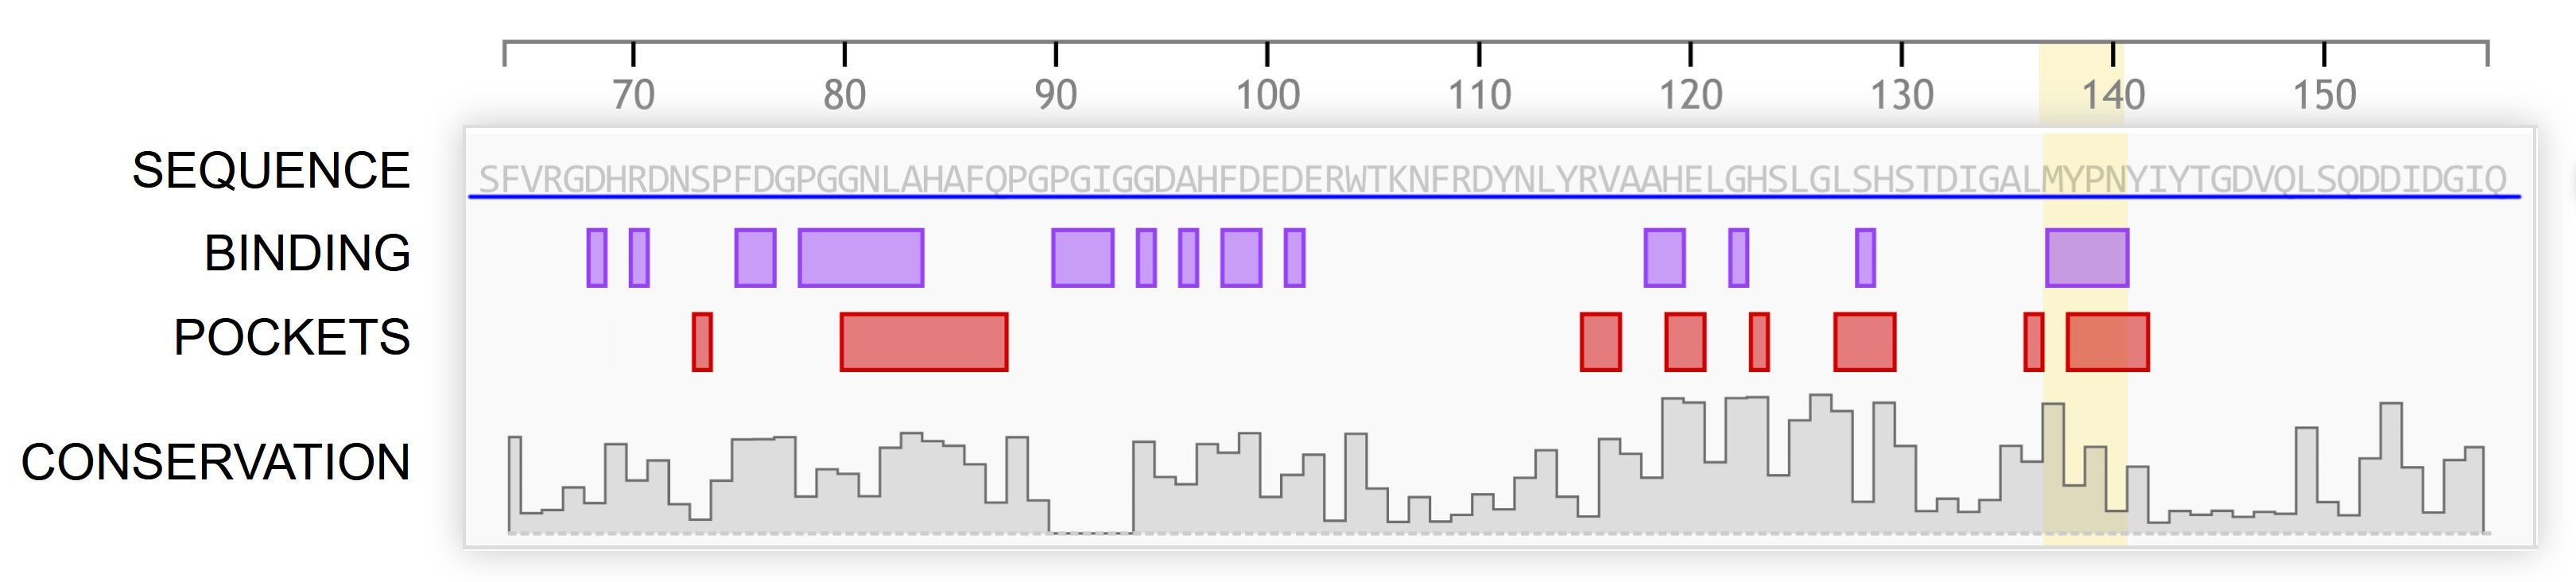
\includegraphics[width=1\linewidth]{primary_done.jpg}
    \caption{Visualization of the primary structure of the 1FBL protein. The sequence of amino acids is underlined in blue. Possible pockets and binding sites predicted by P2Rank are aligned to the sequence and shown in purple and red. Visualization was generated by \href{https://prankweb.cz/viewer?id=1fbl&database=v3-conservation-hmm}{Prank web} (\cite{prankweb}).}
    \label{fig:primary}
\end{figure}

The secondary structure is formed by the folding of the protein. Two primary substructures usually appear as alpha-helix and beta-pleated sheets, visualized in figure ~\ref{fig:secondary} The alpha-helix is a spiral beside the beta-sheet, which refers to folding pieces of the main sequence together. These constitutions are made due to hydrogen bonding between amino and carboxyl groups of peptide bonds in sequence. 

\begin{figure}%
\begin{subfigure}{0.45\textwidth}
    \centering
    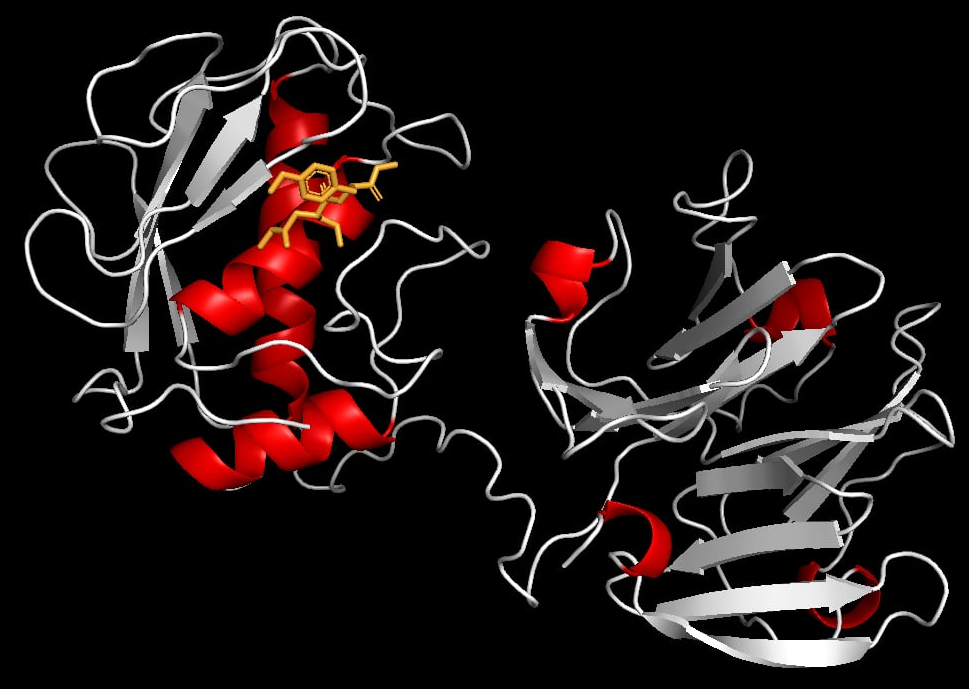
\includegraphics[width=1\linewidth]{alpha_helix.png}
    \caption{Alpha helices}
\end{subfigure}%
\begin{subfigure}{0.45\textwidth}
    \centering
    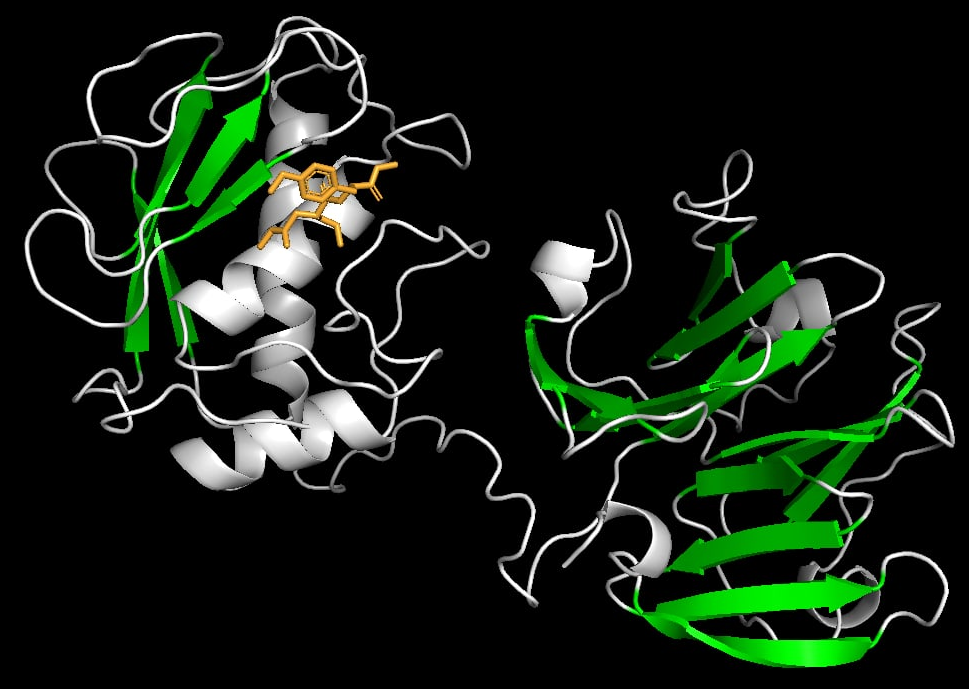
\includegraphics[width=1\linewidth]{beta_sheets.png}
    \caption{Beta sheets}
\end{subfigure}
\caption{Visualization of the secondary structure of the 1FBL protein with an attached ligand. }
\label{fig:secondary}
\end{figure}

The tertiary structure describes the overall three-dimensional arrangement of the molecule. It is determined by the lower substructures and non-covalent interactions, such as intramolecular hydrogen bonding, hydrophilic and hydrophobic interactions, and other non-covalent forces inside the molecule. This structure is essential for binding other molecules called ligands to the protein. It determines whether the surface can form a bond or whether no bond can be created. Data used in this work is described in this structure. This structure can be seen in figure ~\ref{fig:tertiary}.

\begin{figure}
    \centering
    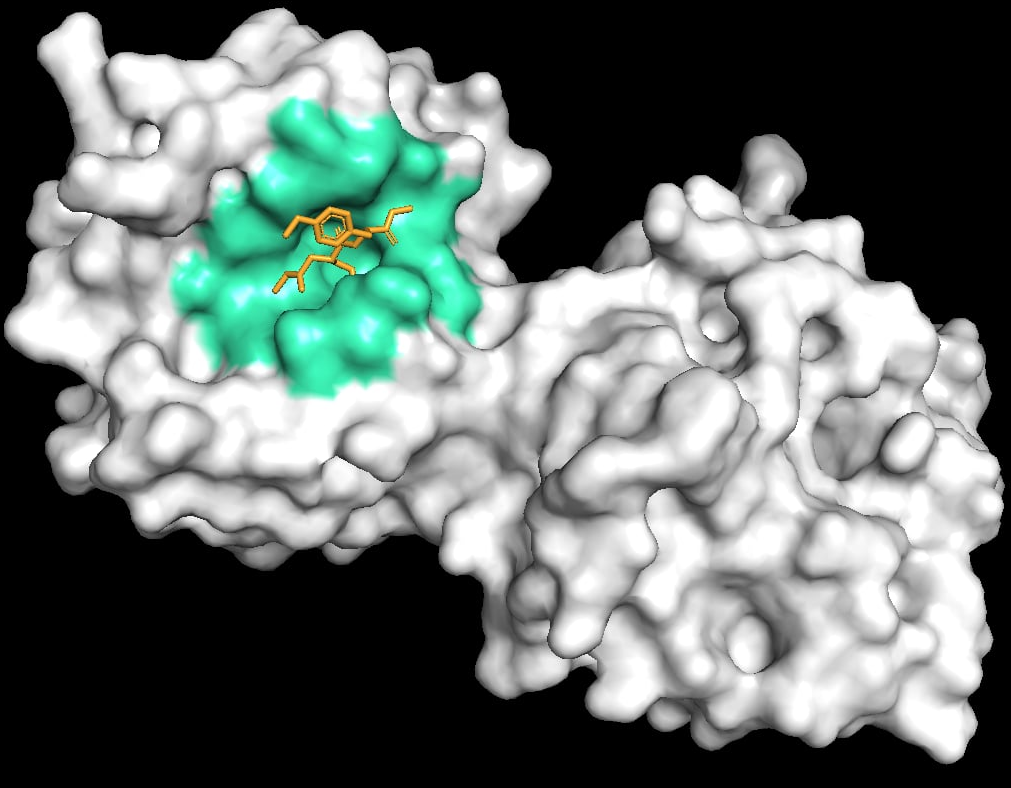
\includegraphics[width=0.5\linewidth]{tertiary.png}
    \caption{Visualization of the tertiary structure of the 1FBL protein with an \ac{LBS} highlighted in cyan with an attached ligand.}
    \label{fig:tertiary}
\end{figure}

Often, the quaternary structure is mentioned in terms of spatial organization. It is the organization of several protein subunits forming an active complex together. For instance, these subunits can be found in hemoglobin, where four molecules with hem create one greater protein complex. This structure is very similar to the tertiary one and irrelevant to the rest of this work.

More detail on this topic can be found in corresponding literature, for example, \cite{kodicek}, from which relevant parts were consulted.

\subsection{SAS points}

P2Rank (\cite{P2RANK}) works with so called \textit{solvent accessible surface} (\ac{SAS}) points. These are points on the surface of the protein (in the tertiary structure point of view), drawn by the estimated radius beyond the water molecule's van der Waals radius, checked afterward, whether they are accessible from the surface or buried in the protein. For these points, different properties can be calculated. These SAS points then form a point cloud used in this work with the described properties acting as per-point features.

\subsection{Ligand Binding Sites}
\label{LBS}

LBSs are parts of the protein where a bond with some ligand can be created. Ligand can be another protein, for instance, a receptor or enzyme. However, the precise definition differs per dataset. The applications for LBS-predictors are best described by \cite{P2RANK}:

\say{%
    Prediction LBS [...] from protein structure has many applications in [the] elucidation of protein function \cite{U1}] and rational drug design [\cite{U2},\cite{U3},\cite{U4}]. It has been employed in drug side-effects prediction [\cite{U5}], fragment-based drug discovery [\cite{U6}], docking prioritization [\cite{U7}, \cite{U8}], structure-based virtual screening [\cite{U9}], and structure-based target prediction (or so-called inverse virtual screening) [\cite{U10}]. Increasingly, LBS prediction is being used in large-scale structural studies that try to analyze and compare all known and putative binding sites on a genome-wide level [\cite{U11},\cite{U12},\cite{U13},\cite{U14},\cite{U15}]. In practice, it is often the case that predicting ligand binding sites is not an end in itself, but it represents only a step in [a] larger automated solution or pipeline.%
    }

In this work, because of limitations caused by the usage of \ac{SAS} points, only LBS on the surface can be detected, although LBS can also be on the inside part of the protein, such as ion binding sites. All the datasets used are constructed with this limitation in mind, and I will not be discussing the non-accessible LBS in this work.
\chapter{Used data}

\section{Raw data intuition}

The raw input into any of our models is the protein's 3D structure. This is represented by a point cloud on the protein's surface. Each point has a feature vector attached, which represents the chemical properties of the given accessible surface patch. Each point also has a ligand-binding class, which the model is used to train and then predict. These can be seen in the figure~\ref{fig:data_point_cloud}.

\begin{figure}
    \centering
    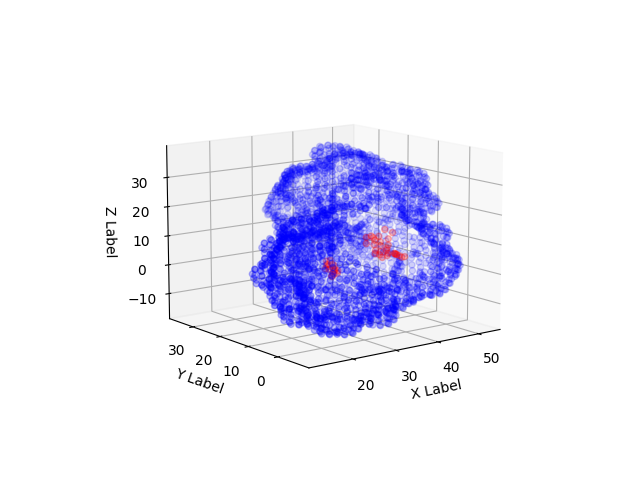
\includegraphics[width=1\linewidth]{img/protein.png}
    \caption{Point cloud with 2 highlighted ligand-binding sites}
    \label{fig:data_point_cloud}
\end{figure}

In the implementation, these points are represented as tabular data, with three columns representing the X, Y, and Z axis, respectively. From this data, the point cloud can be recreated.

\section{Features}

\section{Surroundings extraction}

For the following models, we need to have features for the site's surroundings and the features logged for it.

To achieve this, we run a simple quadratic algorithm for finding the k nearest neighbors. Then, we append their features to the original ones. We use these features instead of the original ones for the following algorithms.

\chapter{Methods}

In this chapter,  firstly, I'm going to describe the interface each method needs to fulfill for a better comparison. Then, I describe the individual models. In the end, I describe the metrics used for comparing the 
\section{Models}
\subsection{Model interface}

All of these models have a common interface of a method  \texttt{predict(protein)}, which takes a protein as an input and returns the predicted probability of each input point being an LBS. For better performance, if not specified otherwise, each model accepts the protein in the surroundings-based format as described in \hyperref[Surroundings]{the corresponding section}. This way, the surroundings dataset can be cached, as the computation of it takes multiple hours.


\subsection{Baseline - small Random Forest Model}
As the first model, we recreate the original model from \cite{P2RANK}. This is the only model that takes the data in the original format. We're using this as a baseline model to compare other models, with the one proposed in the original paper.

This model uses scikit-learn's RandomForestClassifier (RFC) [\cite{scikit-learn}] as a predictor. As described in the original paper, it uses 200 trees with no depth limit and considers a maximum of 6 features in each split. The rest of the parameters are set to default values as described in the \hyperlink{https://scikit-learn.org/1.1/modules/generated/sklearn.ensemble.RandomForestClassifier.html}{corresponding documentation}.


\subsection{Random Forest Model}

Similarly to the Baseline RF model, this model uses an RFC as the predictor. As with all the following models, this one is trained and used on the surroundings dataset. Hyperparameters were tuned using Randomized Parameter Optimization (RPO) from \cite{scikit-learn} with the goal of maximizing the accuracy on a 0.2 validation split. The best hyperparameters found were Tk.

\subsection{PCA + RFC}

Even though RFCs with some modifications can be used for high-dimensional data (such as in \cite{Genuer}), a common approach for handling this case is applying some DM technique as a preprocessing step, most commonly PCA. This is one of the models tested as a baseline to ensure that RFC will not provide falsely low results. PCA's target dimension was handled as a hyperparameter. Using RPO, the best hyperparameters for accuracy on the 0.2 validation set found were Tk.

\subsection{Dense neural network}

Another common approach for classification is dense neural networks (NN). The exact architecture was created by hyperparameter tuning using the Keras Tuner framework towards a 0.2 validation split. The model was optimized using Adam to minimize binary cross-entropy on a 1-unit, sigmoid-activated last layer.

\subsection{REFINED CNN}

This model simplifies an approach proposed by \cite{REFINED}. Compared to the original approach, the DR preprocessing step is skipped. This approach was not tested in the original paper, as some DR method was used in every experiment. The whole algorithm is simplified in the following list. Because this approach is not well known, I'll describe the details in the text following this list. You can see a high-level comparison with the original paper in Figure Tk.

\begin{enumerate}
    \item Input: Set of samples $X = x_1, ... x_n$, where $\forall i x_i \in \mathbb{R}^{D}$, where $D$ is the number of features for each sample (in this case feature vector as described in \hyperref[Surroundings]{the surroundings extraction section}.
    \item We regulize each feature to follow $f \sim N(0,1)$
    \item Reshape each sample to $x_i \in R^{k\times l}$, where $k\cdot l = D$.
    \item We reorder features in the images to create gradients.
    \item Using this permutation, we create a matrix for each sample used in the following step.
    \item We train a CNN on the provided data.
\end{enumerate}

\subsubsection{Pre-REFINED preprocessing}

The first models trained with this approach didn't use any preprocessing. I decided not to recreate the BMDS (or other DR methods) mentioned in the original article. But there was an important part of this step that I didn't account for - feature normalization. This caused issues in the REFINED core and later in the CNN predictions.

Non-normalized data made results from REFINED core visually worse than normalized ones. After explaining the relevant context, I'll discuss why this is the case both in the REFINED core and CNN sections.

After normalization, features are randomly permutated to make this method perform independently in the order of the input features. Then, the vector is reshaped into a matrix of the desired dimensions. 

\subsubsection{REFINED core}

Now comes the interesting part of the algorithm. To allow the location of the feature in the image to have some meaning, we try to minimize over all the permutations of features the value function of 
    $$ f(O|X) = \sum_{s=1}^{n} \sum_{i, j, k, l =1}^n (x^O_{s, ij} - x^O_{s, kl})^2 \cdot \abs{[i,j] - [k,l]}^{-1}$$
Where
\begin{itemize}
    \item $P([D])$ is the set of all permutations on the list of features from $X$,
    \item $F(O|X): P([D]) \rightarrow \mathbb{R}$ is the value function,
    \item $O \in P([D])$ is an ordering of the features
    \item $x^O_s$ is the sample $x_s$ ordered by the ordering $O$
\end{itemize}
Then $x^O_{s, ij}$ is the value is sample $x_s$ on matrix index $[i,j]$ given that the features are ordered by the ordering $O$.

As this is computationally an exponential problem, we approximate this optimum using the hill climbing algorithm (HCA). HCA is not guaranteed to find the optimal permutation. Still, it works well enough as it converges to some local minimum and for convex functions to the global one. I expect that this value function is almost convex (any local minimum will be relatively close to the global one). There isn't a technically viable solution to find the global minimum, as this would require calculating the value function for each permutation (which is $D!$ - or for 900 features $>6\cdot 10^{2269}$). This method was also used in the original paper, so I'm reusing it here.

HCA requires not only the value function $f(X|O)$ but also the neighborhood function $h(O): P([D]) \rightarrow X \in \mathcal{P}(P([D]))$ (output is a subset of $P([D])$ - or a list of orderings). This can be easily computed with the following algorithm:
\begin{lstlisting}
def h(ordering:np.ndarray) -> List[np.ndarray]:
  ret = []
  for i in range(ordering.shape[0]):
    for j in range(ordering.shape[1]):
      for (k, l) in neighboring_pixels(i,j):
        ret.append(swapped(ordering, (i, j), (k, l)))
  return ret

def swapped(array: np.ndarray,
        index0: Tuple[int, int],
        index1: Tuple[int, int]) -> np.ndarray:
    array[index0], array[index1] = array[index1], array[index0]
    return array

def neighboring_pixels(x: int, y: int) -> List[Tuple[int, int]]:
    return [(x + dx, y + dy) 
              for dx in (-1, 0, 1)
              for dy in (-1, 0, 1)
              if (0 <= x + dx < k and 0 <= y + dy < l)
                or not (dx == dy == 0)
            ]
\end{lstlisting}

For complexity's sake, all the neighbors aren't calculated together for the whole ordering, but after each pixel's neighbors are calculated (so for each $i,j$ from the code), we greedily choose the ordering with the lowest value function (or keep the original one, if it is the best) and calculate all the remaining neighbors from this modified state. This increases performance, as we can make as many as $D$ steps per calculation of value functions for the whole ordering neighborhood. But, as it follows the value function's gradient more approximately, it could lead to a higher chance of ending up in a local minimum. Still, this algorithm runs for multiple hours as is, and this can be partly avoided by running multiple HCA's in parallel.

For this work, I used my own Python implementation of HCA to ensure a smoother integration into the rest of the pipeline. Some more tricks were used to improve the speed of the computations, such as using a Numba JIT compiler, or caching value function results. But still, I expect its speed to be lower than some available libraries using C code as the backend.

After this algorithm is finished, we have a feature ordering with correlated features near each other in a generated image and negatively correlated features further away from each other. In Figure Tk., the process of how features are moving can be seen. Also, this can make it easier for humans to see differences between samples compared to looking at the data simply as a vector.

In one of the first experiments, I tried using a genetic evolutionary algorithm (GEA), but it proved to be much slower than the simple HCA - at least with the configuration used then. HCA can be further optimized and run multiple times in parallel, avoiding its pitfalls (getting stuck in a local minimum). Although I didn't succeed with GEA in this part of the algorithm, with some additional work, it might be faster. But this is out of the scope of this work.

As foreshadowed earlier, the REFINED core does not work well with non-normalized data. This can be easily explained. The REFINED core works by aligning correlated features together. However, to make the process easier, only the $L2$ norm of the difference between each feature is computed. This causes features with different means to be further away from each other. Not only that, it causes features with higher variations to be further away from each other. Small differences between low-variational features then influence the value function very little, compared to high-variational features with vastly different means. However, this is not useful information for the predictor following this step.


%  https://www.nature.com/articles/s41598-021-90923-y#citeas
\section{Evaluation Criteria}

Every method was evaluated in terms of speed and performance criteria. In the following part, I will describe the process of gathering these metrics.

All time-related metrics were gathered on an AMD Ryzen 7 PRO 5850U without GPU acceleration.

\subsection{Training Wall Time}

The training wall time measures the wall time for training a model with already set hyperparameters. We do not include the hyperparameter tuning as for different models, different spaces need to be covered, and a different framework is used for optimizing RFC models and Neural Network-based ones.

The time counter starts just before initializing the untrained model and ends directly after training has ended. This means that evaluation of the model on the test set is not included in this metric, but validation during the training is (e.g., per epoch validation in (C)NN training).

\subsection{Inference Wall Time}

As training is done only once per model lifespan, but inference happens on every model usage, inference time could be much more important depending on the use case.

This time is measured during test-set evaluation and measures only the time the model runs on the whole dataset. This doesn't include metric evaluation of the results, model loading into memory, or any other task.

\subsection{Model performance metrics}

Because all used datasets are imbalanced (97 \% of samples are negative), the f1-score is used as the main evaluation metric. However, accuracy, precision, recall, and false positive rate (FPR) are all calculated. Given that $TP$ is the number of true positives, $FP$ false positives, $TN$ true negatives and $FN$ false positives, aforementioned metrics are defined as follows:
$$F_1 = \frac{2TP}{2TP + FP + FN}$$
$$Accuracy = \frac{TP + TN}{TP + FP + TN + FN}$$
$$Precision = \frac{TP}{TP + FP}$$
$$Recall = \frac{TP}{TP + FN}$$
$$FPR = \frac{FP}{FP + TN}$$

For each dataset, a per protein value of each metric is calculated. Then, a 95 \% interval is created for the mean value. These are then plotted to show a comparison.
\chapter{Experiments}

\section{Overall comparison}

The main experiment consists of comparing all the methods in their whole pipeline. First, I run hyperparameter optimization for each method as described in its description. Then, with these hyperparameters, a model is trained. The \textit{chen11} dataset is used for training, and metrics are calculated on the \textit{coach420} dataset.

With this experiment, I want to test whether REFINED performs better on this dataset than other state-of-the-art approaches. 
\begin{figure}
    \centering
    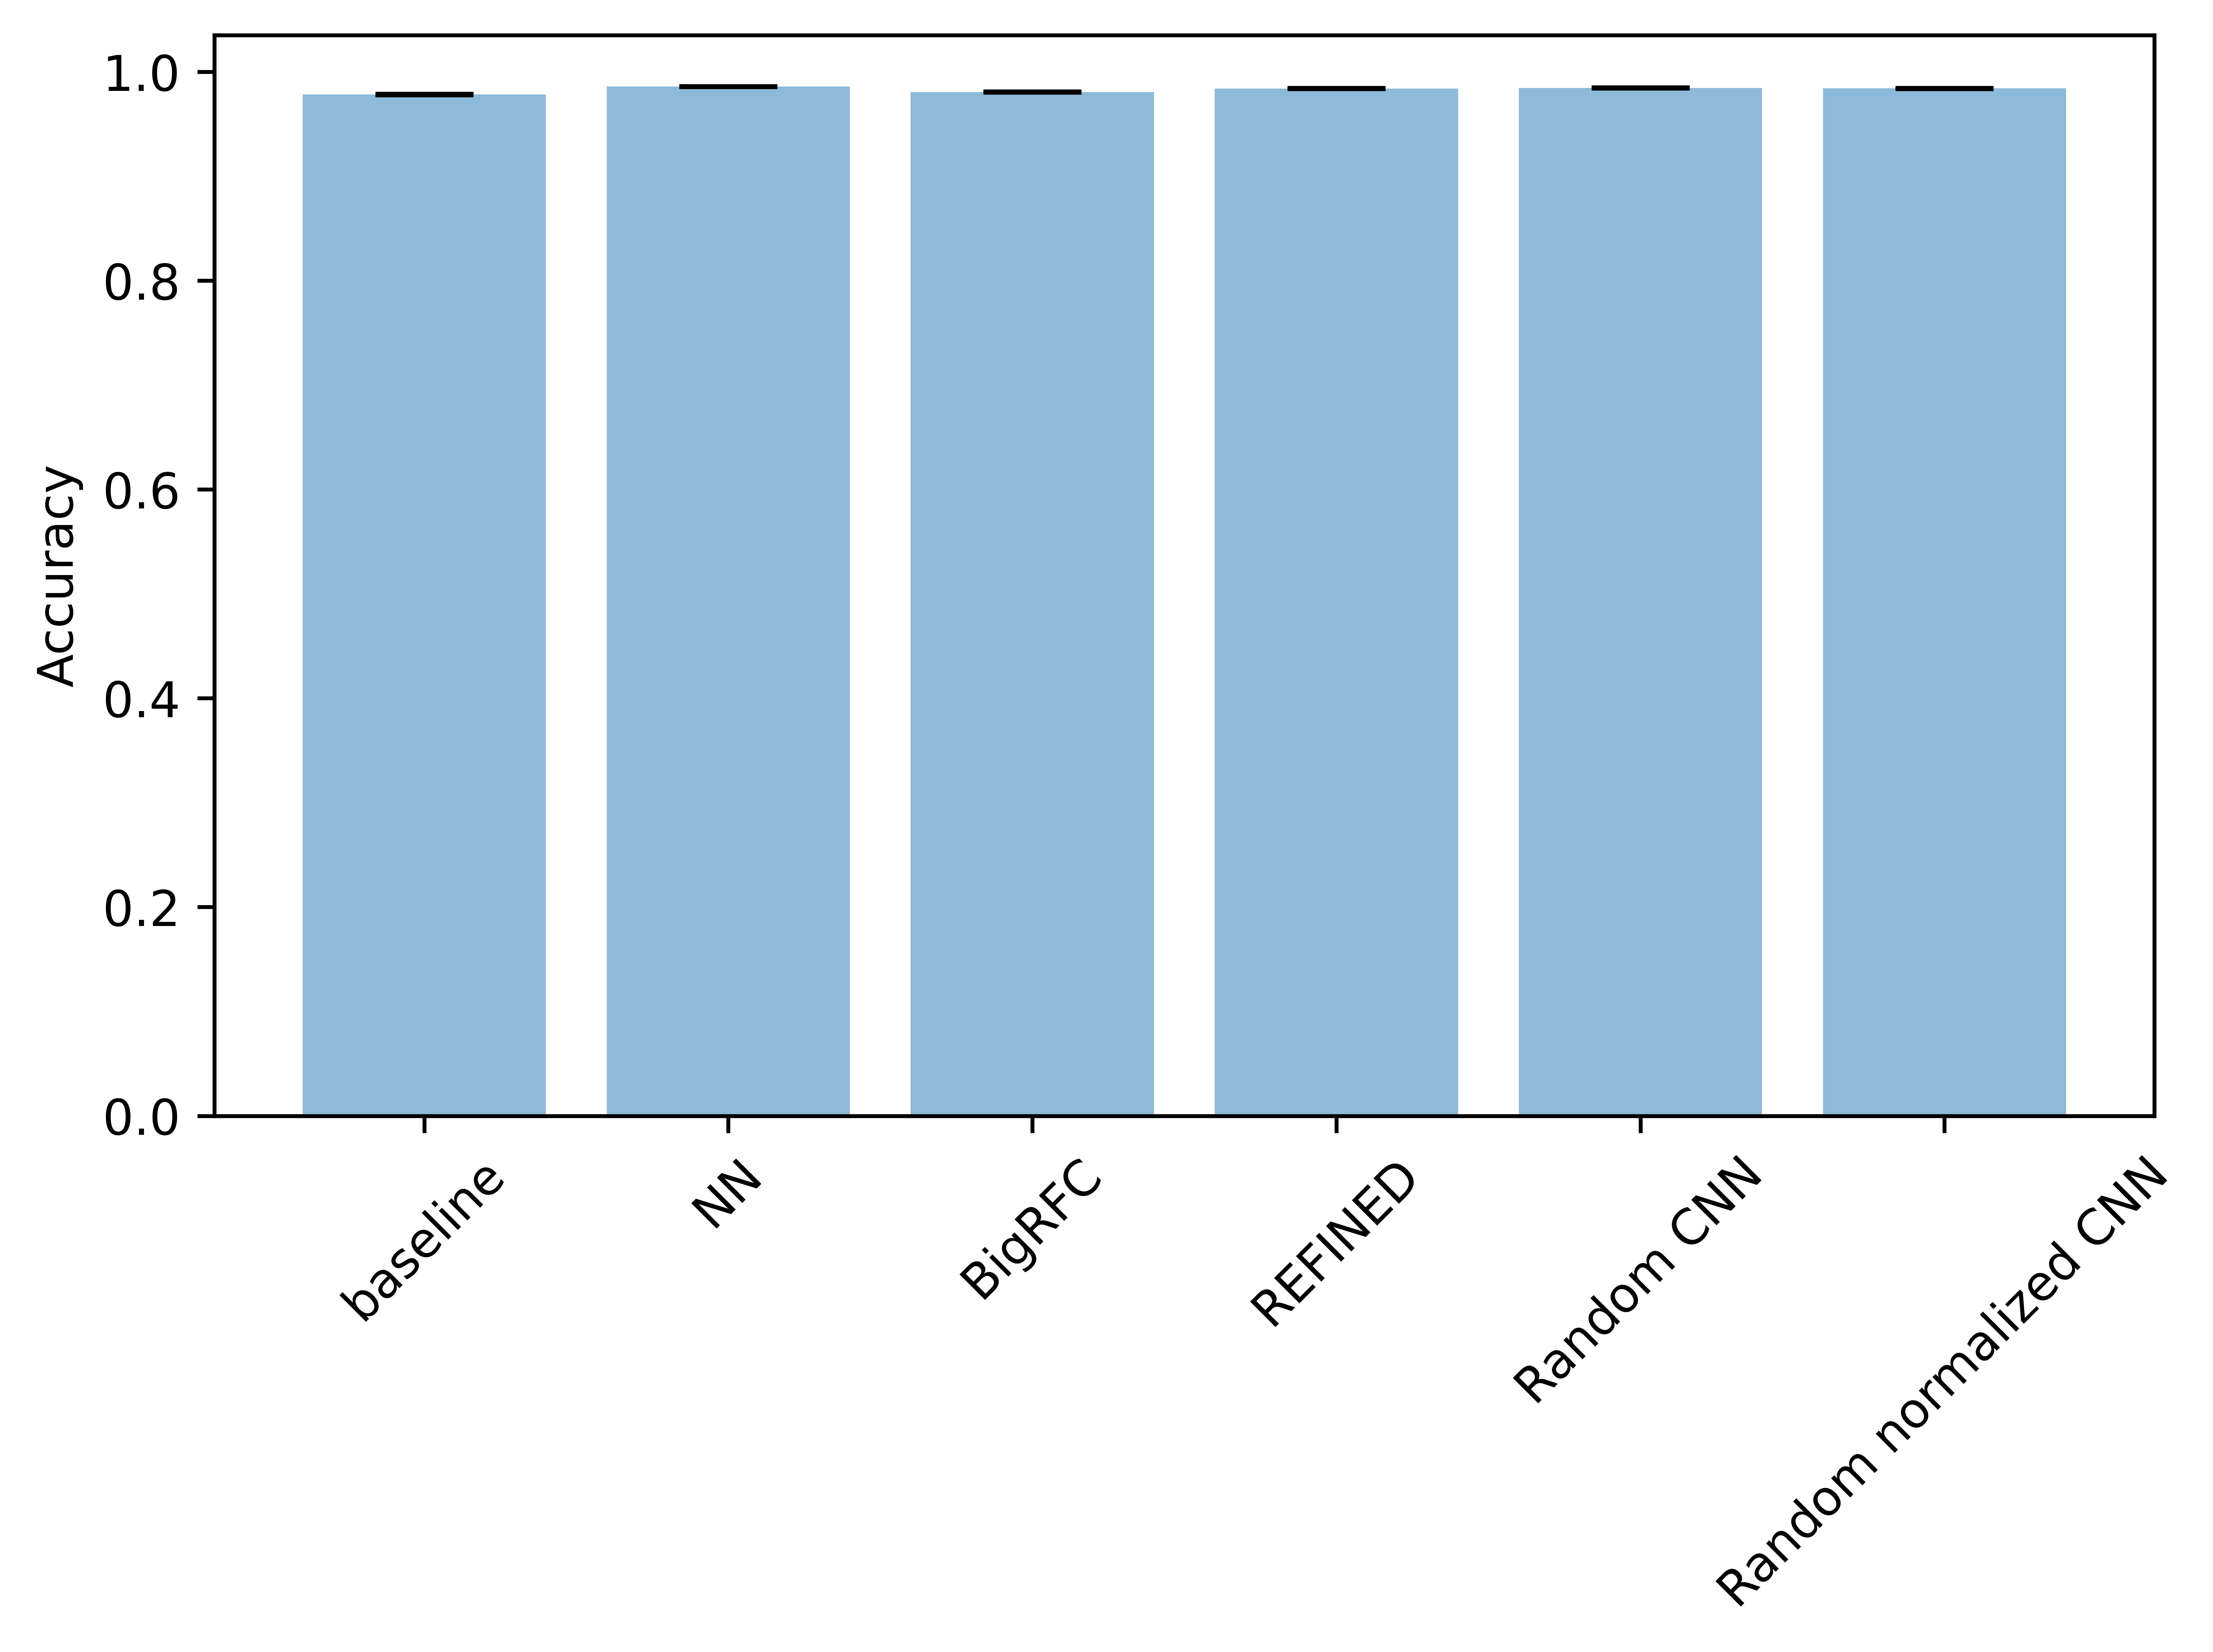
\includegraphics[width=0.5\linewidth]{img/Accuracy.png}
    \caption{Accuracy measurements for all models}
    \label{fig:accuracy}
\end{figure}
\begin{figure}
    \centering
    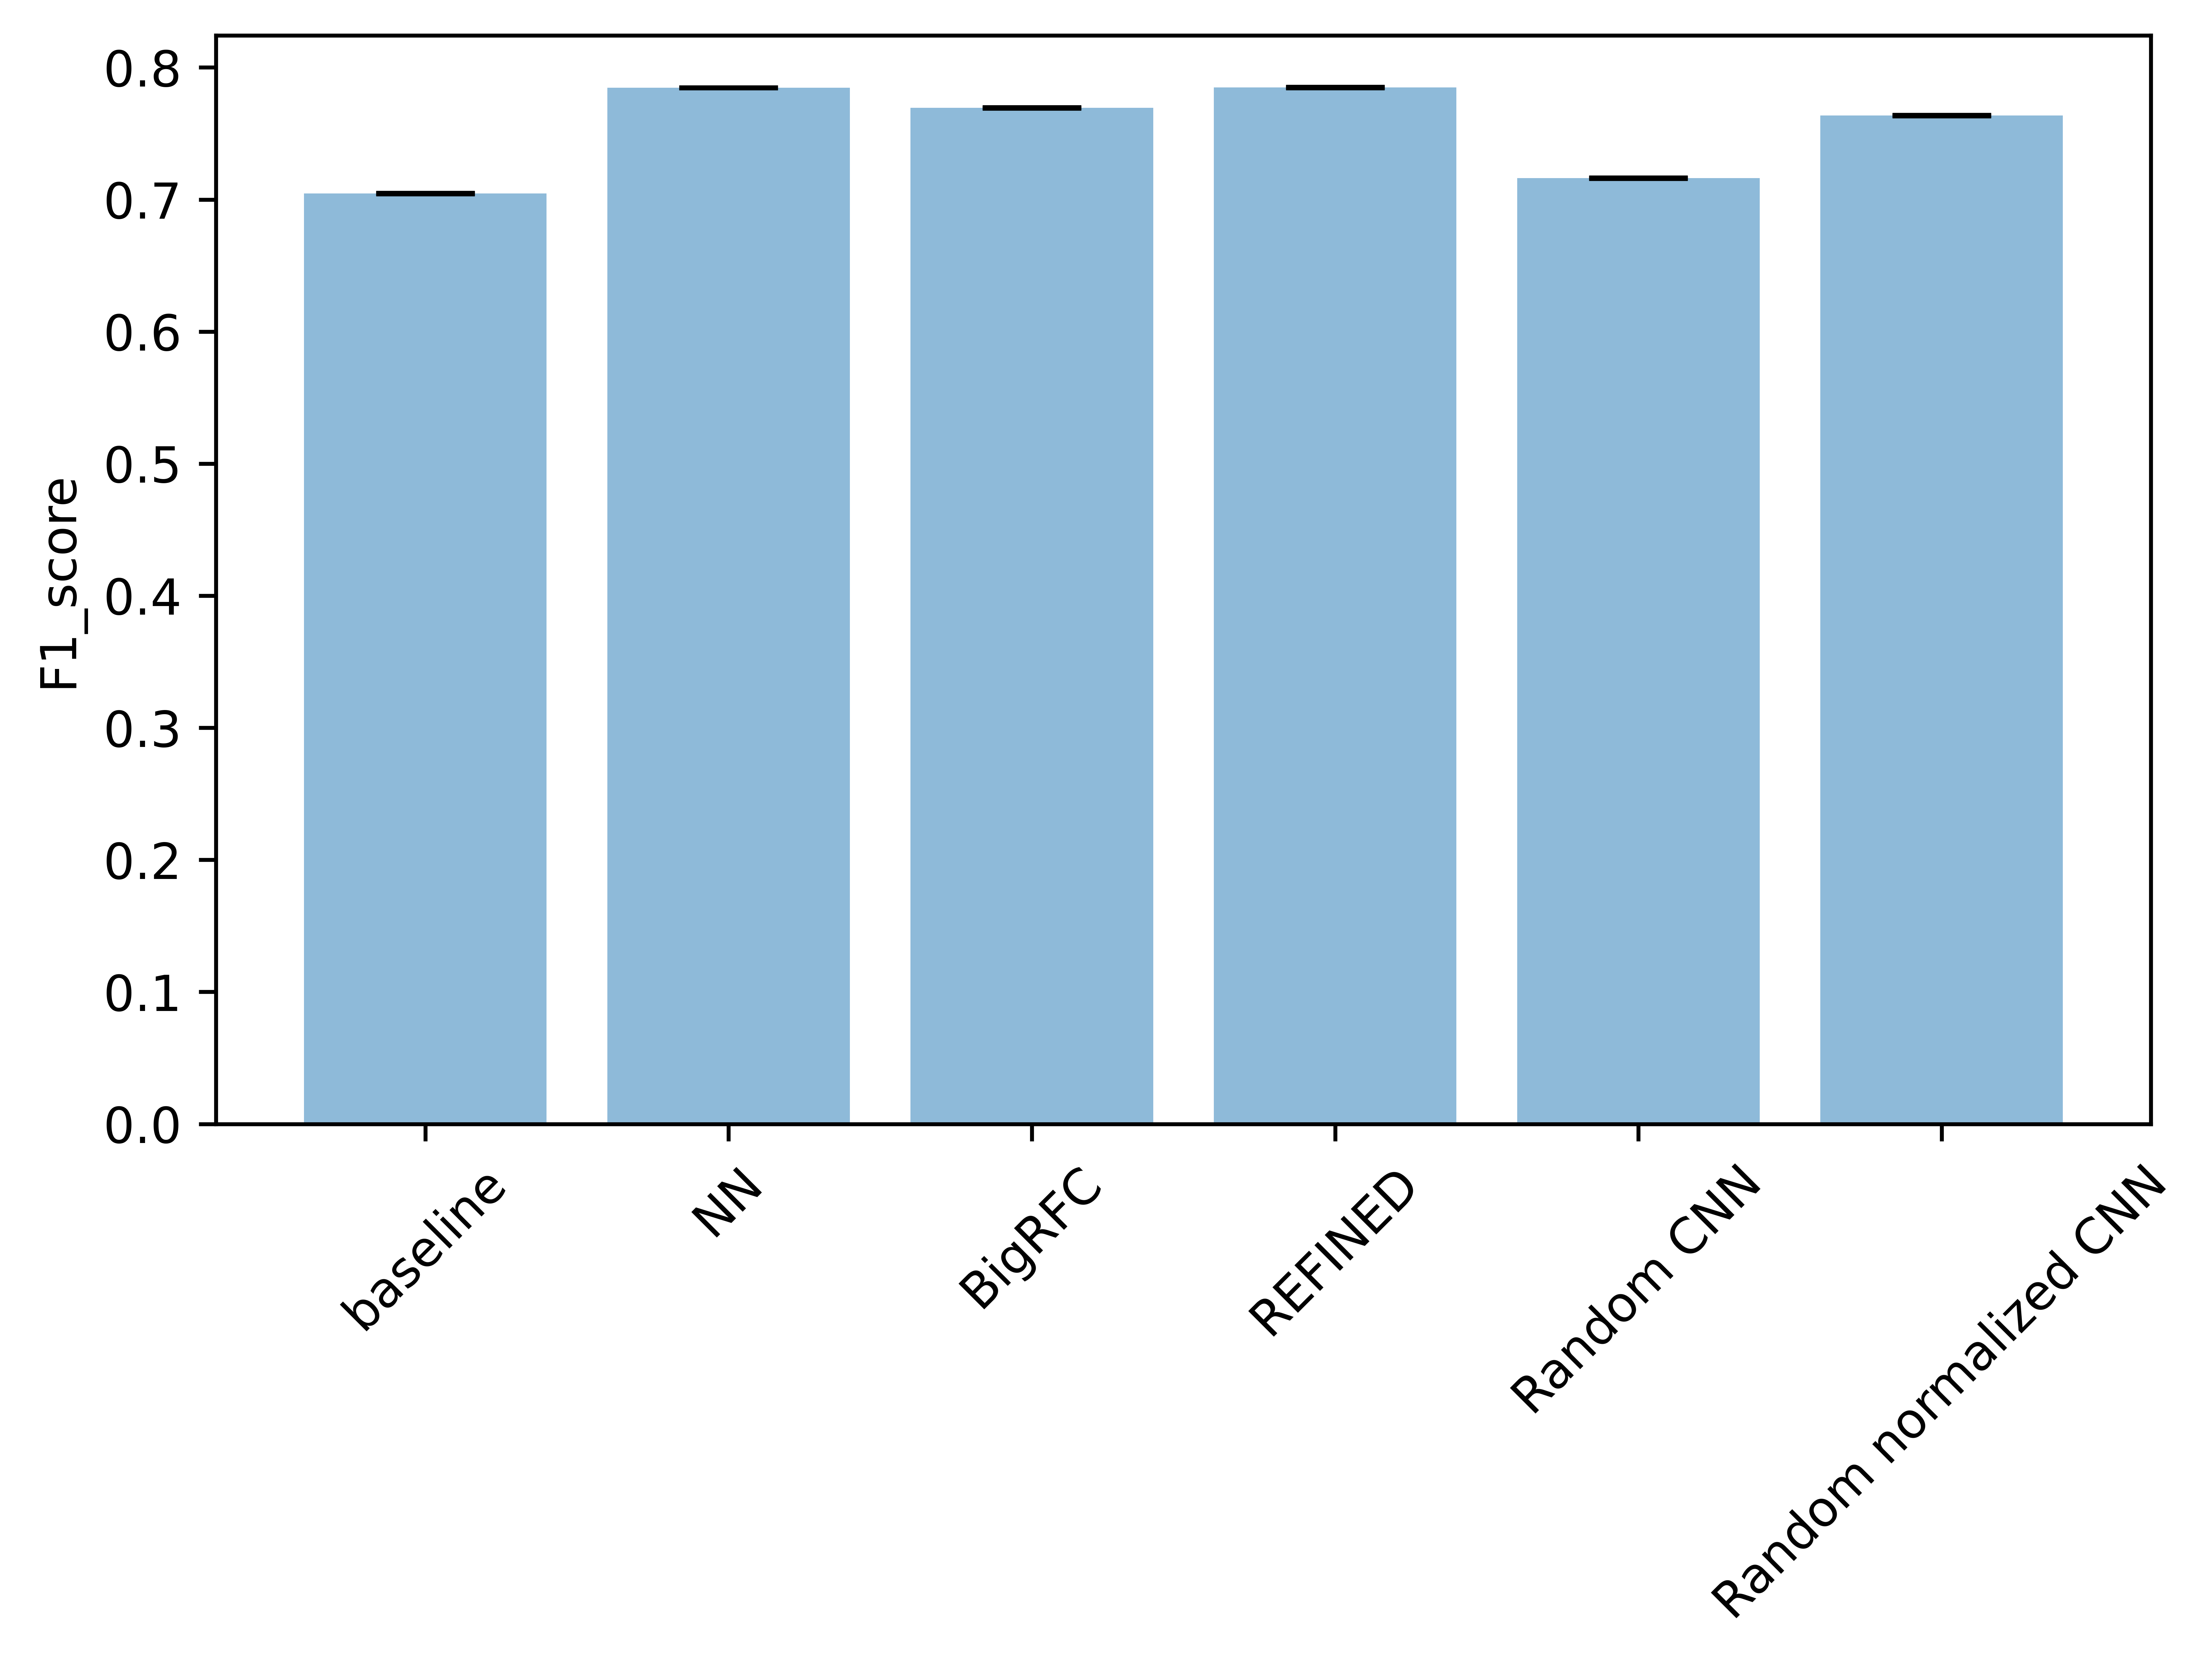
\includegraphics[width=0.5\linewidth]{F1_score.png}
    \caption{F1 scores for all models}
    \label{fig:f1}
\end{figure}

\begin{figure}
    \centering
    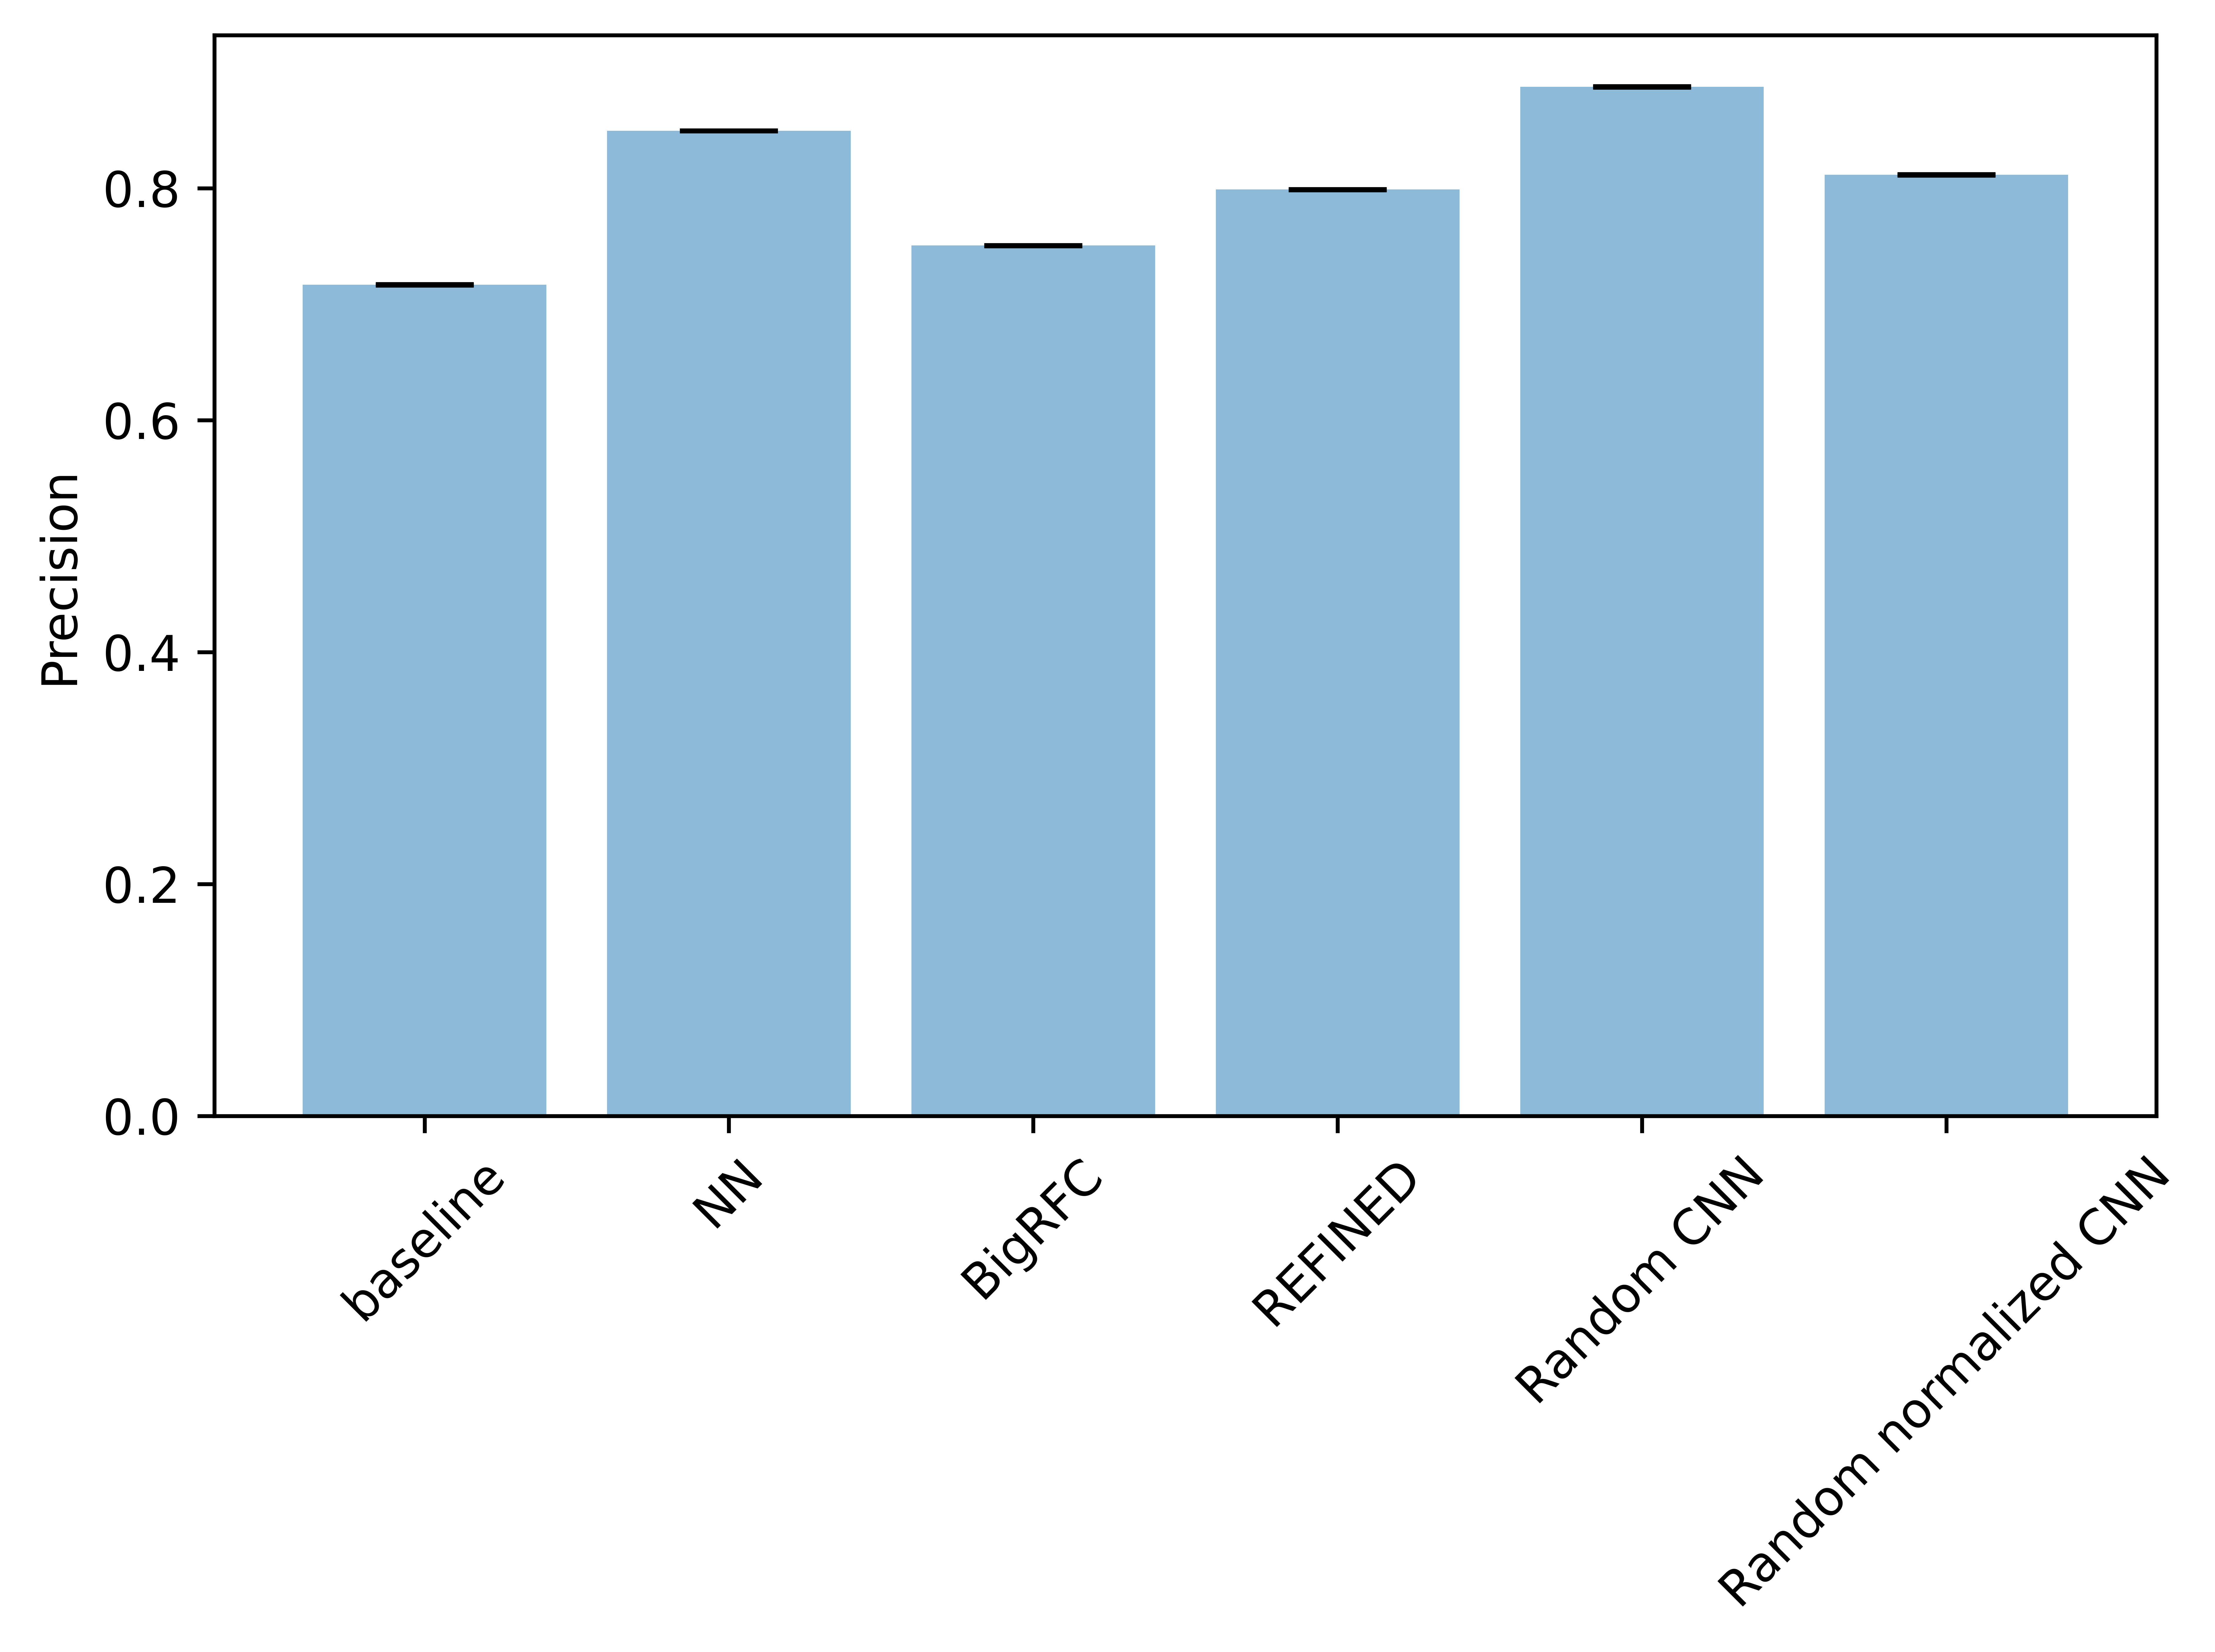
\includegraphics[width=0.5\linewidth]{Precision.png}
    \caption{Precision for all models}
    \label{fig:precision}
\end{figure}

\begin{figure}
    \centering
    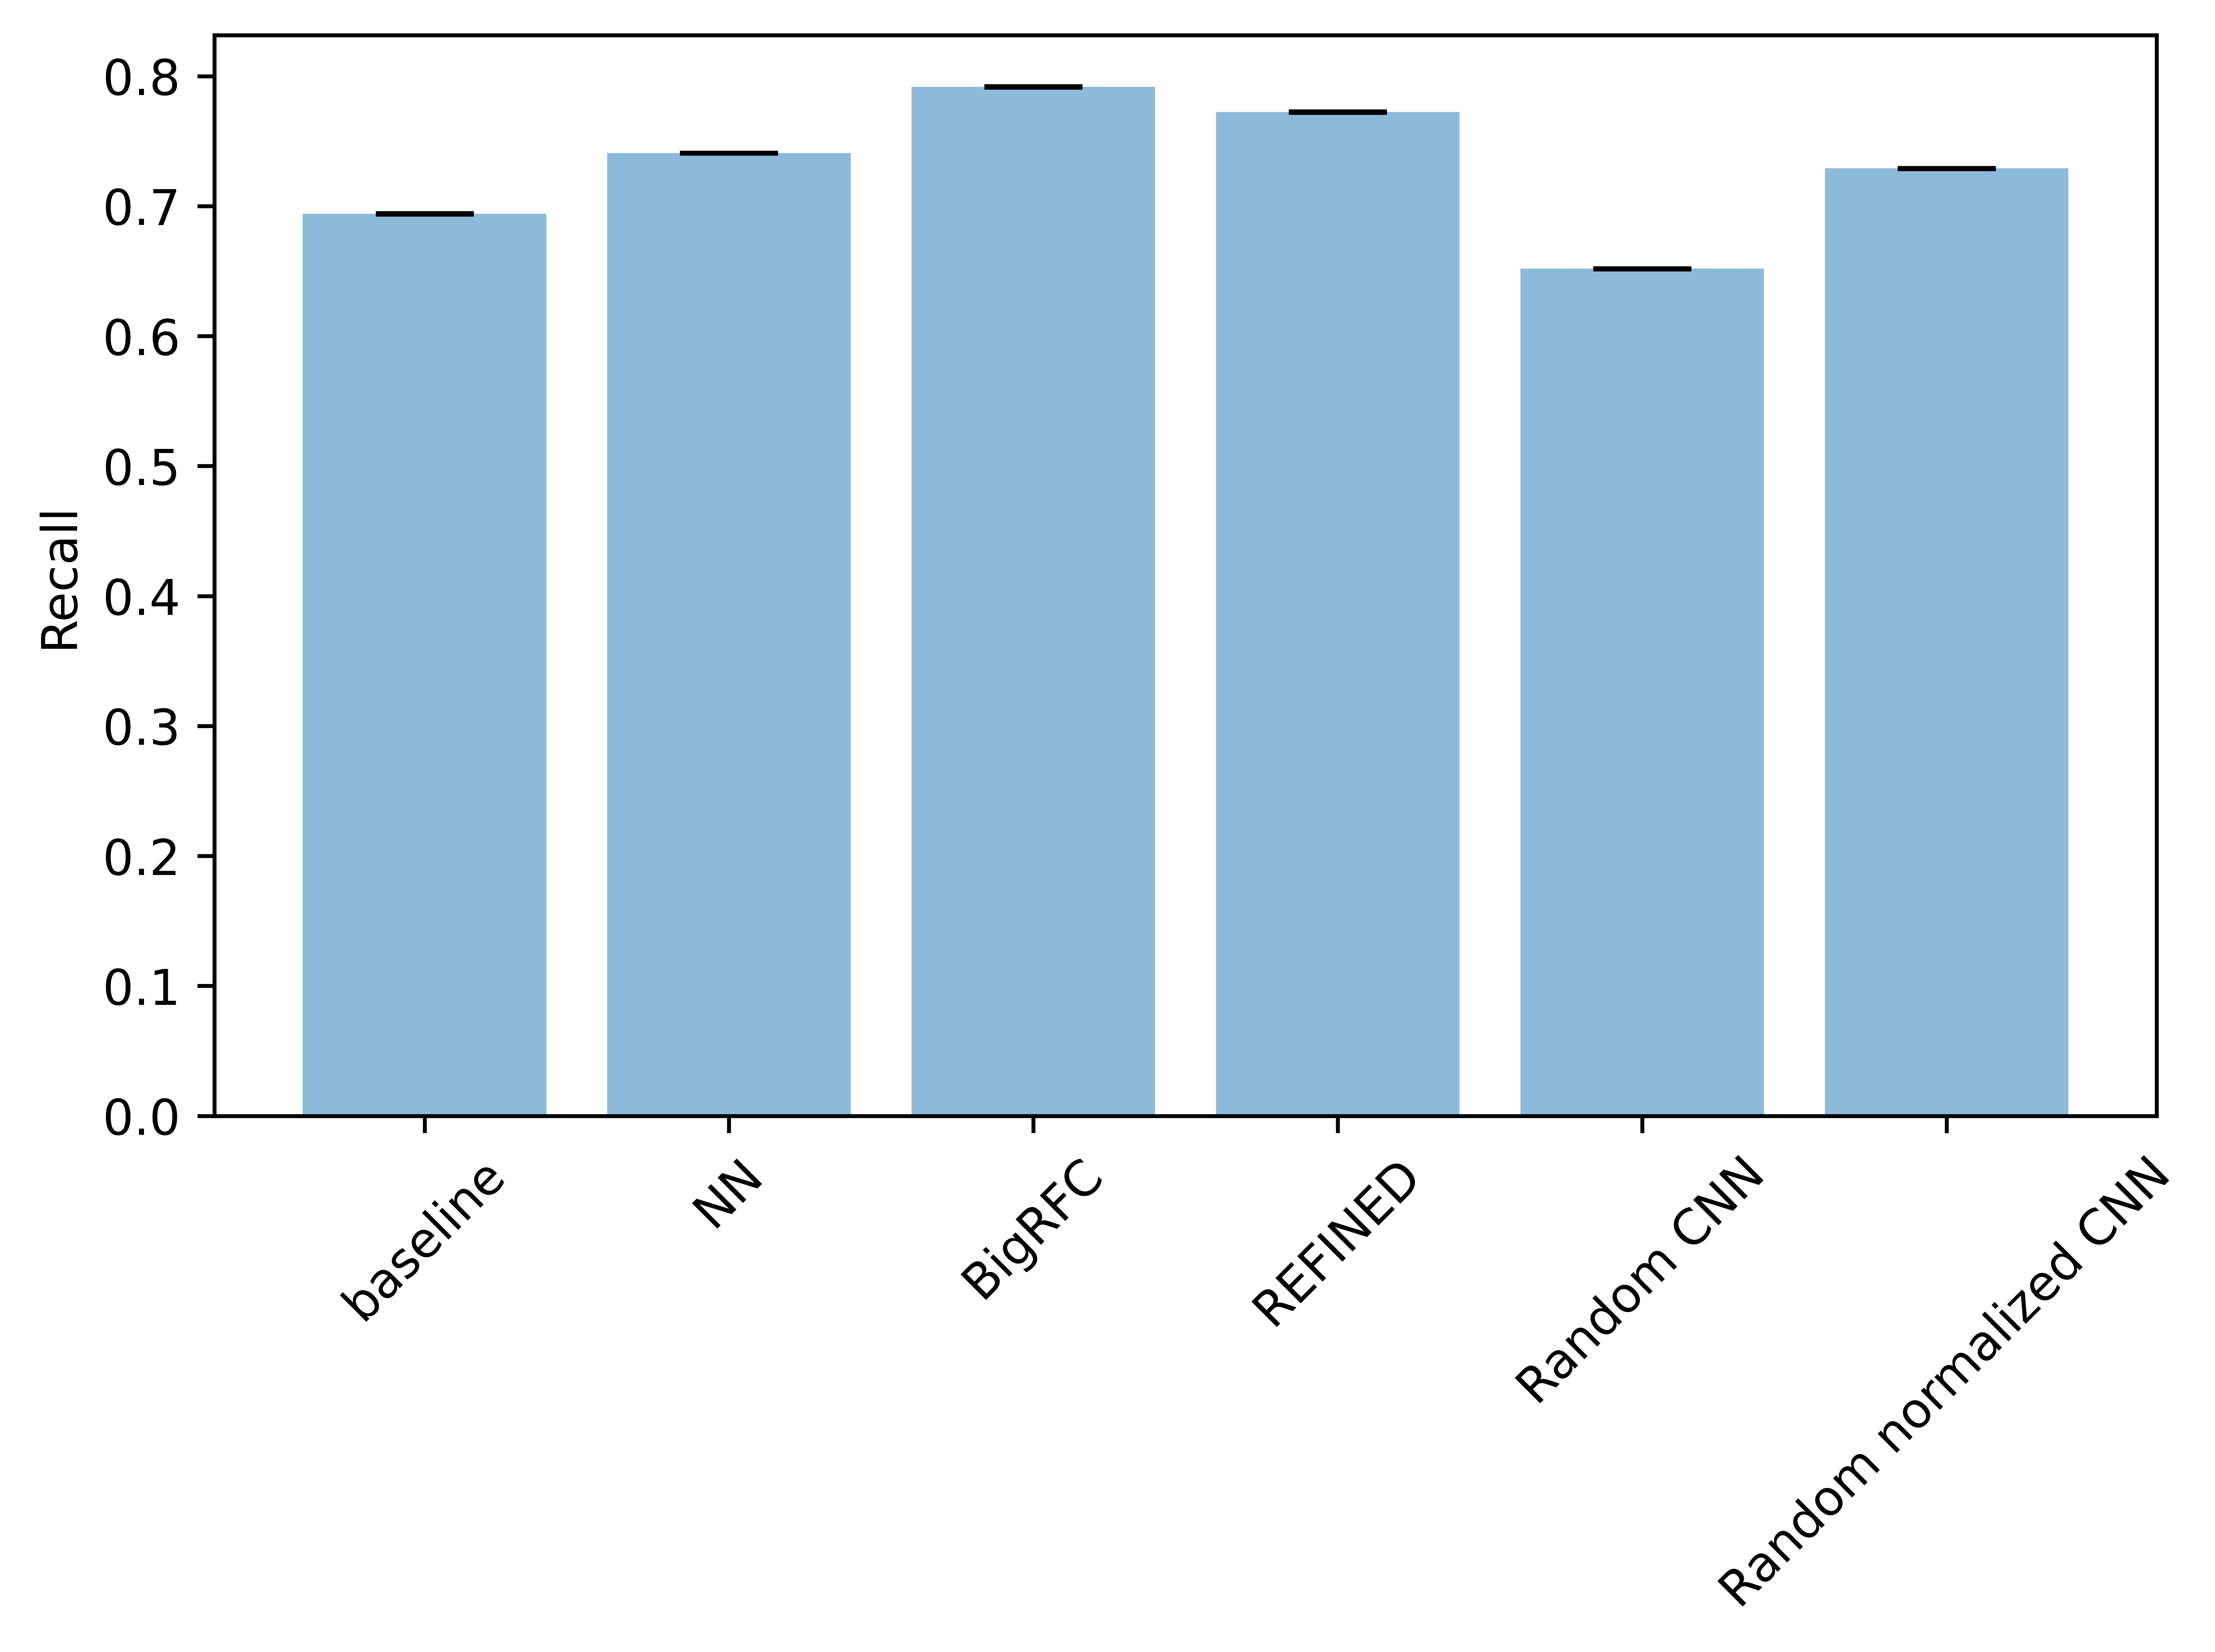
\includegraphics[width=0.5\linewidth]{Recall.png}
    \caption{Recall for all models}
    \label{fig:recall}
\end{figure}

As can be seen in the attached figures (~\ref{fig:accuracy}, ~\ref{fig:precision}, ~\ref{fig:f1}, ~\ref{fig:recall}) REFINED model is on par with state-of-the-art approaches, but does not bring higher performance as reported in \cite{REFINED}. However, it shows better results than Random CNN and even Random Normalized CNN.

\section{REFINED progression test}

With the negative results of the previous test, I wanted to test whether training a CNN on REFINED-transformed images produces better results than on images with randomly allocated positions. I have taken the individual epochs of REFINED and trained a CNN model on it to test this. The models are called \texttt{CNN-i}, where \texttt{i} is the number of epochs of REFINED used as input. So \texttt{CNN-0} will have features distributed very closely to randomly and \texttt{CNN-43} is a fully trained REFINED model. All of these models were trained using CNN hyperparameters found for the REFINED model in the first experiment.

Then, I tested whether there was any correlation between the REFINED score and CNN's performance. The obvious metric to compare is the validation loss, as it represents the training goals the best.

\begin{figure}
    \centering
    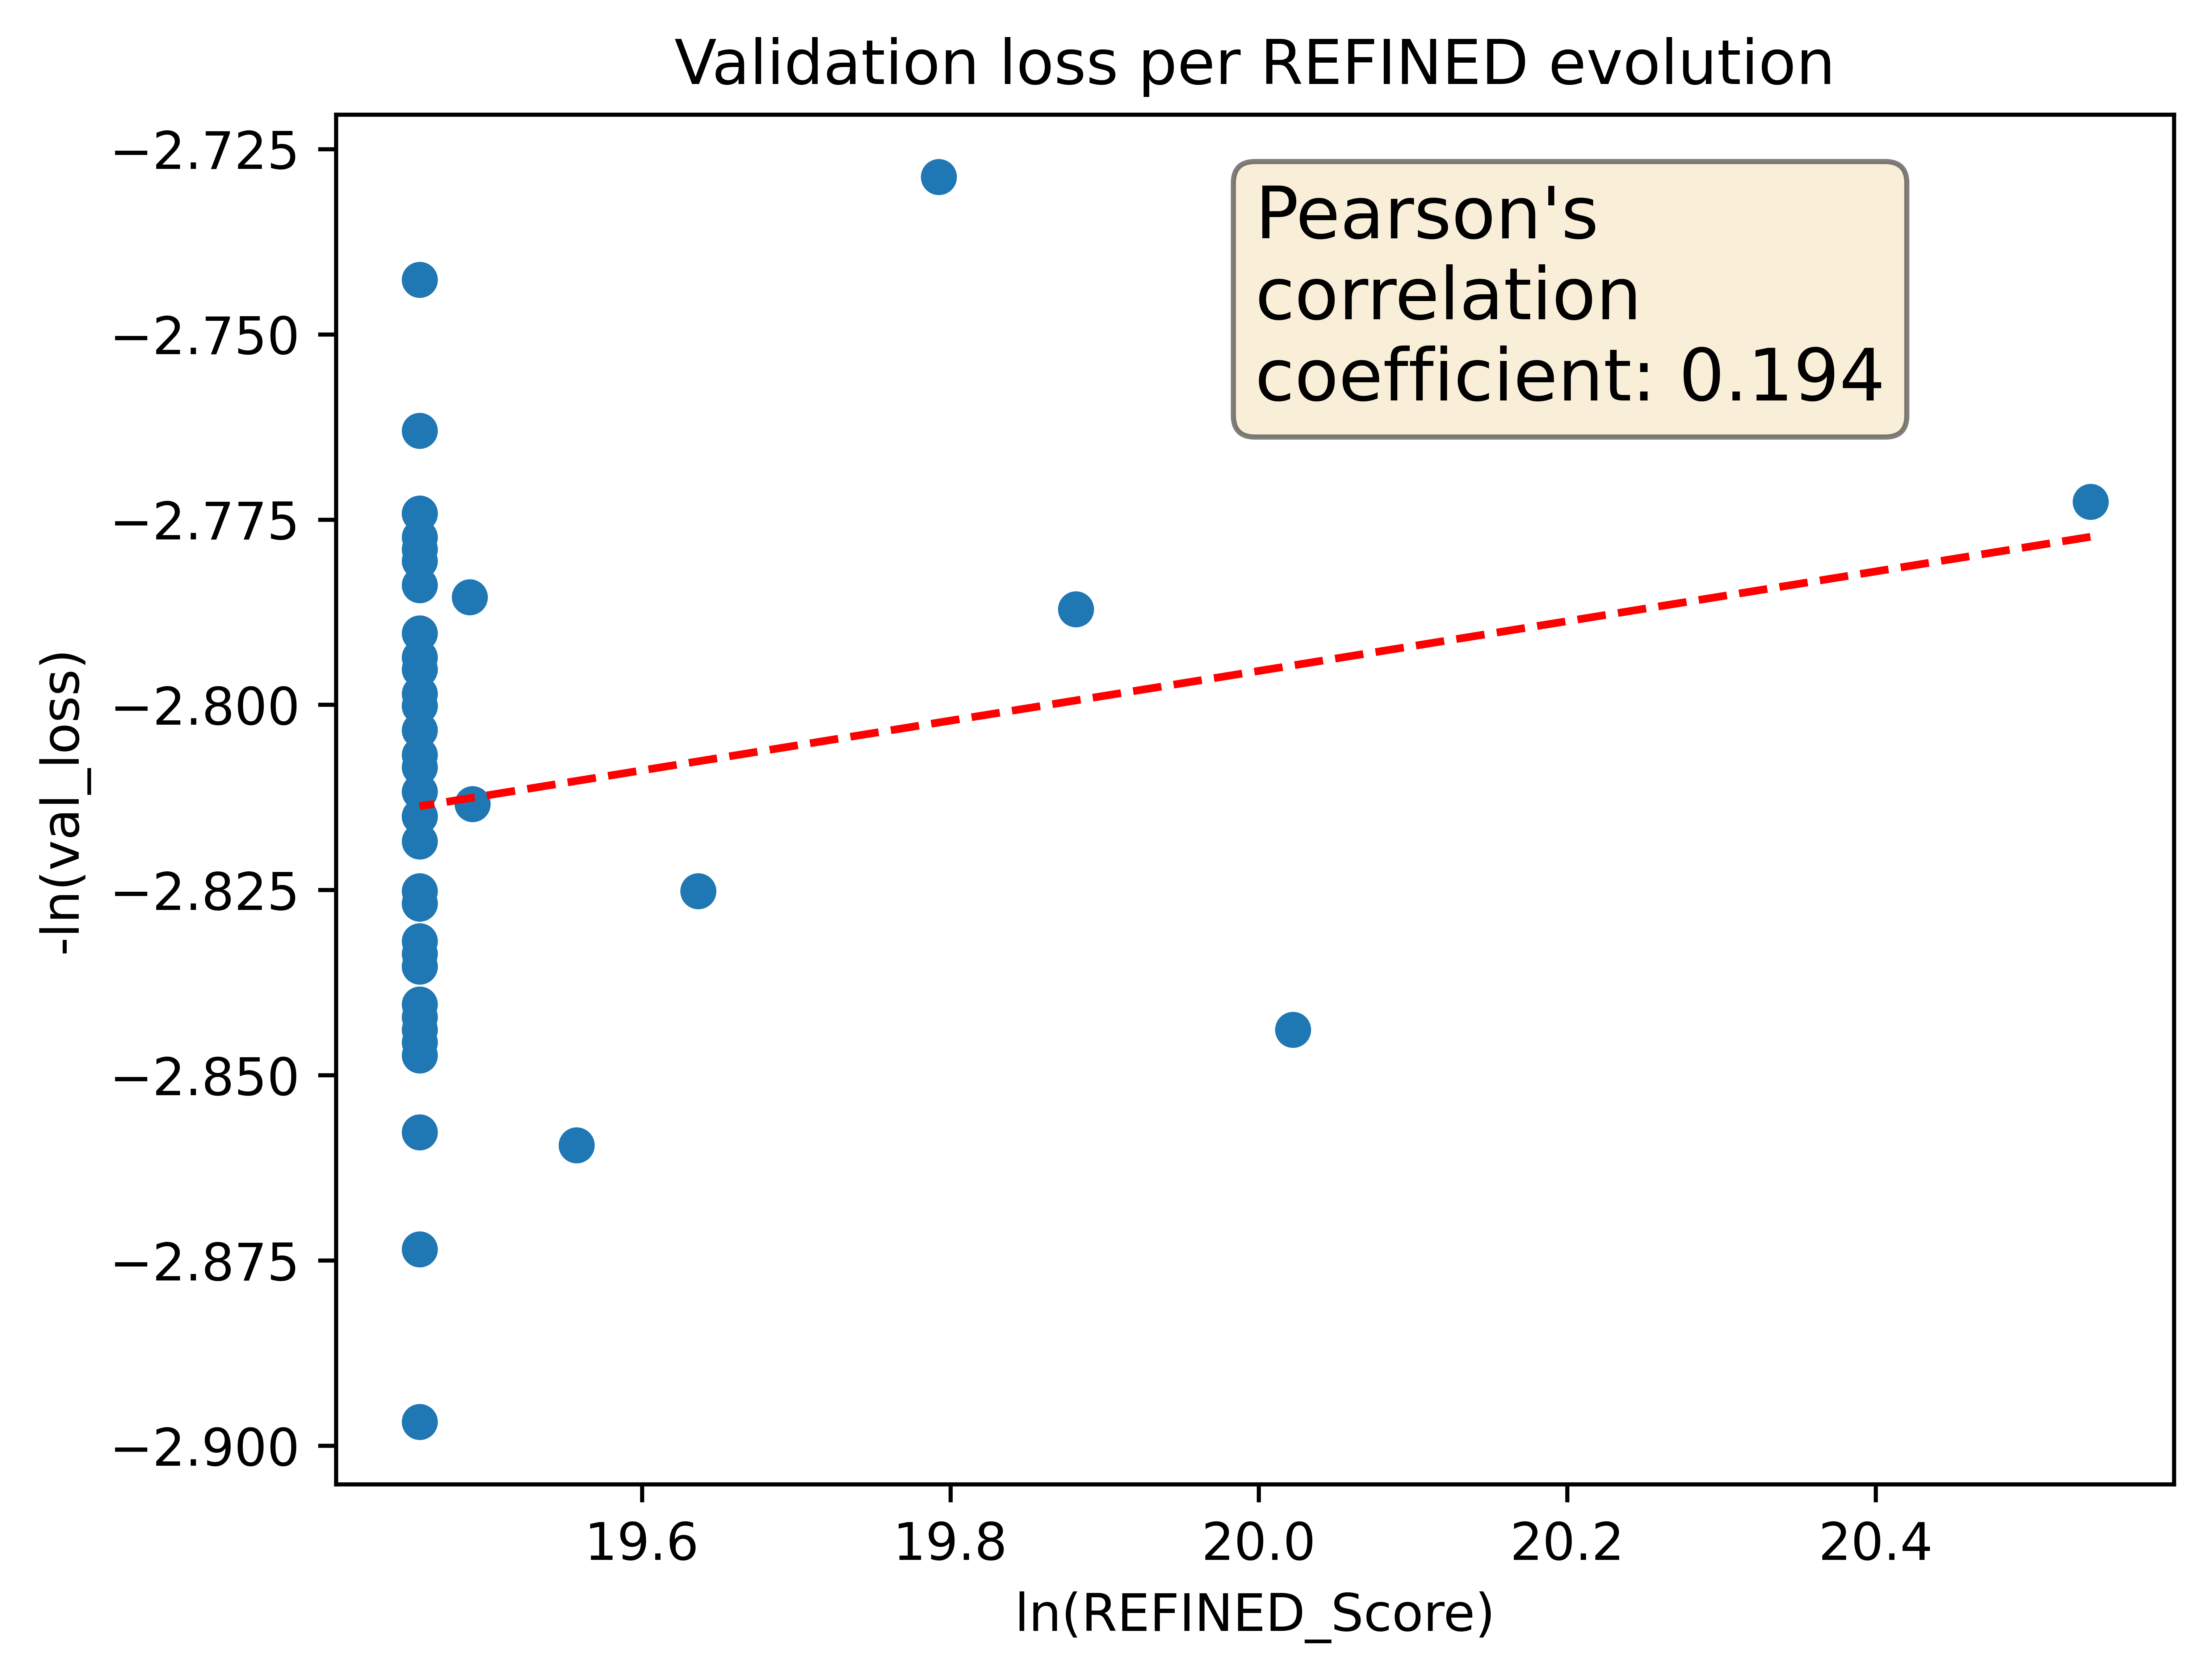
\includegraphics[width=0.5\linewidth]{progression.png}
    \caption{Best CNN validation loss plotted against }
    \label{fig:REFINED_progression}
\end{figure}

In ~\ref{fig:REFINED_progression} can be seen that there is little to no correlation between the REFINED score and the model's performance.

\section{REFINED transformation visualized}
At the beginning of this thesis, one of the motivations for this work was the interest in seeing high-dimensional data visualised in some manner. And REFINED does achieve that goal. 
\chapter{Discussion}

\section{Meaning of the results}

\section{Steps that didn't seem to go anywhere}

% \chapter*{Conclusion}
\addcontentsline{toc}{chapter}{Conclusion}
In this work, I explored the potential of convolutional neural networks (CNNs) for detecting protein-ligand binding sites, specifically focusing on the REFINED algorithm's ability to transform high-dimensional feature vectors into images suitable for CNN analysis. While previous research suggested promising results with this approach, the findings of this thesis did not provide significant evidence to support the superiority of REFINED over established methods.

The experiments conducted on the CHEN11 and COACH420 datasets revealed that:
\begin{itemize}
    \item \textbf{REFINED} did not show a significant improvement in predictive power compared to state-of-the-art approaches, such as Random Forest Classifiers or dense neural networks.*While REFINED successfully rearranged features into images with visual gradients, this did not translate into a demonstrable advantage in binding site prediction accuracy.
    \item \textbf{No correlation was found between the REFINED score and the performance of CNN models trained on the resulting images.} This suggests that REFINED's specific arrangement of features does not inherently enhance CNN's ability to identify binding sites.

\end{itemize}

While the primary hypothesis of this thesis was not confirmed, valuable insights were gained:
\begin{itemize}
    \item \textbf{The importance of considering surrounding features for accurate binding site prediction was confirmed.} Models utilizing the surrounding context of each point, such as the RFC Surrounding and NN models, achieved better performance compared to the P2Rank RFC model that solely relied on individual point features.
    \item \textbf{The potential of CNNs in this domain remains open for further exploration.} Future research could investigate alternative methods for feature vector transformation or different CNN architectures that might better capture the spatial relationships relevant to protein-ligand interactions. 

\end{itemize}

In conclusion, although the anticipated benefits of REFINED were not observed in this study, the exploration of CNNs for binding site prediction offered valuable insights into the complexities of this problem. The findings suggest that while considering the surrounding context of each point is crucial, the specific arrangement of features within images may not be the determining factor for achieving optimal performance. Future research should continue to investigate the potential of CNNs and alternative approaches to advance the field of protein-ligand binding site prediction. \footnote{Writing of the conclusion chapter has been assisted by the Gemini 1.5 Ultra. The writing of the whole work has been assisted by \href{https://www.grammarly.com/premium}{Grammarly} writing assistant. All usage of AI tools was conducted in accordance with the Code of Ethics of the Faculty of Mathematics and Physics of Charles University.}


%%% Bibliography
%%% Bibliography (literature used as a source)
%%%
%%% We employ bibTeX to construct the bibliography. It processes
%%% citations in the text (e.g., the \cite{...} macro) and looks up
%%% relevant entries in the bibliography.bib file.
%%%
%%% The \bibliographystyle command selects, which style will be used
%%% for references from the text. The argument in curly brackets is
%%% the name of the corresponding style file (*.bst). Both styles
%%% mentioned in this template are included in LaTeX distributions.

\bibliographystyle{plainnat}    %% Author (year)
% \bibliographystyle{unsrt}     %% [number]

\renewcommand{\bibname}{Bibliography}

%%% Generate the bibliography. Beware that if you cited no works,
%%% the empty list will be omitted completely.

\bibliography{bibliography}

%%% If case you prefer to write the bibliography manually (without bibTeX),
%%% you can use the following. Please follow the ISO 690 standard and
%%% citation conventions of your field of research.

% \begin{thebibliography}{99}
%
% \bibitem{lamport94}
%   {\sc Lamport,} Leslie.
%   \emph{\LaTeX: A Document Preparation System}.
%   2nd edition.
%   Massachusetts: Addison Wesley, 1994.
%   ISBN 0-201-52983-1.
%
% \end{thebibliography}


%%% Figures used in the thesis (consider if this is needed)
\listoffigures

%%% Tables used in the thesis (consider if this is needed)
%%% In mathematical theses, it could be better to move the list of tables to the beginning of the thesis.
% \listoftables

%%% Abbreviations used in the thesis, if any, including their explanation
%%% In mathematical theses, it could be better to move the list of abbreviations to the beginning of the thesis.
% \chapwithtoc{List of Abbreviations}

%%% Attachments to the bachelor thesis, if any. Each attachment must be
%%% referred to at least once from the text of the thesis. Attachments
%%% are numbered.
%%%
%%% The printed version should preferably contain attachments, which can be
%%% read (additional tables and charts, supplementary text, examples of
%%% program output, etc.). The electronic version is more suited for attachments
%%% which will likely be used in an electronic form rather than read (program
%%% source code, data files, interactive charts, etc.). Electronic attachments
%%% should be uploaded to SIS and optionally also included in the thesis on a~CD/DVD.
%%% Allowed file formats are specified in provision of the rector no. 72/2017.
\appendix
% \chapter{Attachments}

% \section{First Attachment}

\openright
\end{document}
